\documentclass[twoside]{book}

% Packages required by doxygen
\usepackage{fixltx2e}
\usepackage{calc}
\usepackage{doxygen}
\usepackage[export]{adjustbox} % also loads graphicx
\usepackage{graphicx}
\usepackage[utf8]{inputenc}
\usepackage{makeidx}
\usepackage{multicol}
\usepackage{multirow}
\PassOptionsToPackage{warn}{textcomp}
\usepackage{textcomp}
\usepackage[nointegrals]{wasysym}
\usepackage[table]{xcolor}

% Font selection
\usepackage[T1]{fontenc}
\usepackage[scaled=.90]{helvet}
\usepackage{courier}
\usepackage{amssymb}
\usepackage{sectsty}
\renewcommand{\familydefault}{\sfdefault}
\allsectionsfont{%
  \fontseries{bc}\selectfont%
  \color{darkgray}%
}
\renewcommand{\DoxyLabelFont}{%
  \fontseries{bc}\selectfont%
  \color{darkgray}%
}
\newcommand{\+}{\discretionary{\mbox{\scriptsize$\hookleftarrow$}}{}{}}

% Page & text layout
\usepackage{geometry}
\geometry{%
  a4paper,%
  top=2.5cm,%
  bottom=2.5cm,%
  left=2.5cm,%
  right=2.5cm%
}
\tolerance=750
\hfuzz=15pt
\hbadness=750
\setlength{\emergencystretch}{15pt}
\setlength{\parindent}{0cm}
\setlength{\parskip}{0.2cm}
\makeatletter
\renewcommand{\paragraph}{%
  \@startsection{paragraph}{4}{0ex}{-1.0ex}{1.0ex}{%
    \normalfont\normalsize\bfseries\SS@parafont%
  }%
}
\renewcommand{\subparagraph}{%
  \@startsection{subparagraph}{5}{0ex}{-1.0ex}{1.0ex}{%
    \normalfont\normalsize\bfseries\SS@subparafont%
  }%
}
\makeatother

% Headers & footers
\usepackage{fancyhdr}
\pagestyle{fancyplain}
\fancyhead[LE]{\fancyplain{}{\bfseries\thepage}}
\fancyhead[CE]{\fancyplain{}{}}
\fancyhead[RE]{\fancyplain{}{\bfseries\leftmark}}
\fancyhead[LO]{\fancyplain{}{\bfseries\rightmark}}
\fancyhead[CO]{\fancyplain{}{}}
\fancyhead[RO]{\fancyplain{}{\bfseries\thepage}}
\fancyfoot[LE]{\fancyplain{}{}}
\fancyfoot[CE]{\fancyplain{}{}}
\fancyfoot[RE]{\fancyplain{}{\bfseries\scriptsize Generated on Wed Apr 27 2016 23\+:33\+:32 for Ridesharing by Doxygen }}
\fancyfoot[LO]{\fancyplain{}{\bfseries\scriptsize Generated on Wed Apr 27 2016 23\+:33\+:32 for Ridesharing by Doxygen }}
\fancyfoot[CO]{\fancyplain{}{}}
\fancyfoot[RO]{\fancyplain{}{}}
\renewcommand{\footrulewidth}{0.4pt}
\renewcommand{\chaptermark}[1]{%
  \markboth{#1}{}%
}
\renewcommand{\sectionmark}[1]{%
  \markright{\thesection\ #1}%
}

% Indices & bibliography
\usepackage{natbib}
\usepackage[titles]{tocloft}
\setcounter{tocdepth}{3}
\setcounter{secnumdepth}{5}
\makeindex

% Hyperlinks (required, but should be loaded last)
\usepackage{ifpdf}
\ifpdf
  \usepackage[pdftex,pagebackref=true]{hyperref}
\else
  \usepackage[ps2pdf,pagebackref=true]{hyperref}
\fi
\hypersetup{%
  colorlinks=true,%
  linkcolor=blue,%
  citecolor=blue,%
  unicode%
}

% Custom commands
\newcommand{\clearemptydoublepage}{%
  \newpage{\pagestyle{empty}\cleardoublepage}%
}


%===== C O N T E N T S =====

\begin{document}

% Titlepage & ToC
\hypersetup{pageanchor=false,
             bookmarks=true,
             bookmarksnumbered=true,
             pdfencoding=unicode
            }
\pagenumbering{roman}
\begin{titlepage}
\vspace*{7cm}
\begin{center}%
{\Large Ridesharing }\\
\vspace*{1cm}
{\large Generated by Doxygen 1.8.10}\\
\vspace*{0.5cm}
{\small Wed Apr 27 2016 23:33:32}\\
\end{center}
\end{titlepage}
\clearemptydoublepage
\tableofcontents
\clearemptydoublepage
\pagenumbering{arabic}
\hypersetup{pageanchor=true}

%--- Begin generated contents ---
\chapter{Hierarchical Index}
\section{Class Hierarchy}
This inheritance list is sorted roughly, but not completely, alphabetically\+:\begin{DoxyCompactList}
\item \contentsline{section}{App}{\pageref{class_app}}{}
\item \contentsline{section}{Car}{\pageref{class_car}}{}
\item \contentsline{section}{Connection}{\pageref{class_connection}}{}
\item \contentsline{section}{Crossroad}{\pageref{class_crossroad}}{}
\item \contentsline{section}{Edge$<$ T, U $>$}{\pageref{class_edge}}{}
\item \contentsline{section}{Edge\+Type}{\pageref{class_edge_type}}{}
\item \contentsline{section}{File\+Reading\+Error}{\pageref{class_file_reading_error}}{}
\item \contentsline{section}{Graph$<$ T, U $>$}{\pageref{class_graph}}{}
\item \contentsline{section}{Graph$<$ Crossroad, Road $>$}{\pageref{class_graph}}{}
\begin{DoxyCompactList}
\item \contentsline{section}{Road\+Map}{\pageref{class_road_map}}{}
\end{DoxyCompactList}
\item \contentsline{section}{Graph\+Viewer}{\pageref{class_graph_viewer}}{}
\item \contentsline{section}{Ride}{\pageref{class_ride}}{}
\begin{DoxyCompactList}
\item \contentsline{section}{Ride\+Offer}{\pageref{class_ride_offer}}{}
\item \contentsline{section}{Ride\+Request}{\pageref{class_ride_request}}{}
\end{DoxyCompactList}
\item \contentsline{section}{Ride\+Completed}{\pageref{class_ride_completed}}{}
\item \contentsline{section}{Road}{\pageref{class_road}}{}
\item \contentsline{section}{User}{\pageref{class_user}}{}
\item \contentsline{section}{Vertex$<$ T, U $>$}{\pageref{class_vertex}}{}
\item \contentsline{section}{vertex\+\_\+greater\+\_\+than$<$ T, U $>$}{\pageref{structvertex__greater__than}}{}
\item \contentsline{section}{Wrong\+File\+Parameters}{\pageref{class_wrong_file_parameters}}{}
\end{DoxyCompactList}

\chapter{Class Index}
\section{Class List}
Here are the classes, structs, unions and interfaces with brief descriptions\+:\begin{DoxyCompactList}
\item\contentsline{section}{\hyperlink{class_app}{App} }{\pageref{class_app}}{}
\item\contentsline{section}{\hyperlink{class_car}{Car} }{\pageref{class_car}}{}
\item\contentsline{section}{\hyperlink{class_connection}{Connection} }{\pageref{class_connection}}{}
\item\contentsline{section}{\hyperlink{class_crossroad}{Crossroad} }{\pageref{class_crossroad}}{}
\item\contentsline{section}{\hyperlink{class_edge}{Edge$<$ T, U $>$} }{\pageref{class_edge}}{}
\item\contentsline{section}{\hyperlink{class_edge_type}{Edge\+Type} }{\pageref{class_edge_type}}{}
\item\contentsline{section}{\hyperlink{class_file_reading_error}{File\+Reading\+Error} }{\pageref{class_file_reading_error}}{}
\item\contentsline{section}{\hyperlink{class_graph}{Graph$<$ T, U $>$} }{\pageref{class_graph}}{}
\item\contentsline{section}{\hyperlink{class_graph_viewer}{Graph\+Viewer} }{\pageref{class_graph_viewer}}{}
\item\contentsline{section}{\hyperlink{class_ride}{Ride} }{\pageref{class_ride}}{}
\item\contentsline{section}{\hyperlink{class_ride_completed}{Ride\+Completed} }{\pageref{class_ride_completed}}{}
\item\contentsline{section}{\hyperlink{class_ride_offer}{Ride\+Offer} }{\pageref{class_ride_offer}}{}
\item\contentsline{section}{\hyperlink{class_ride_request}{Ride\+Request} }{\pageref{class_ride_request}}{}
\item\contentsline{section}{\hyperlink{class_road}{Road} }{\pageref{class_road}}{}
\item\contentsline{section}{\hyperlink{class_road_map}{Road\+Map} }{\pageref{class_road_map}}{}
\item\contentsline{section}{\hyperlink{class_user}{User} }{\pageref{class_user}}{}
\item\contentsline{section}{\hyperlink{class_vertex}{Vertex$<$ T, U $>$} }{\pageref{class_vertex}}{}
\item\contentsline{section}{\hyperlink{structvertex__greater__than}{vertex\+\_\+greater\+\_\+than$<$ T, U $>$} }{\pageref{structvertex__greater__than}}{}
\item\contentsline{section}{\hyperlink{class_wrong_file_parameters}{Wrong\+File\+Parameters} }{\pageref{class_wrong_file_parameters}}{}
\end{DoxyCompactList}

\chapter{Class Documentation}
\hypertarget{class_app}{}\section{App Class Reference}
\label{class_app}\index{App@{App}}
\subsection*{Public Member Functions}
\begin{DoxyCompactItemize}
\item 
\hyperlink{class_app_acb8cbf3e285b91d0170ffe87df5989c5}{App} ()
\item 
void \hyperlink{class_app_ab996c03e3b8455a98c3ee32684353bf4}{read\+Data} (string filename)
\item 
void \hyperlink{class_app_a22ee53e2dc589184357e31a61bbb1bbc}{read\+Data\+Rides} (string filename)
\item 
void \hyperlink{class_app_a726ada082015afbaf04b4f2bcc4dbd6d}{add\+User} (string name, string address)
\item 
void \hyperlink{class_app_ac03ffaeef9892bec7f6b304c647073c9}{add\+Ride\+Request} (\hyperlink{class_user}{User} $\ast$user, uint departure\+Place, uint arrival\+Place, time\+\_\+t departure\+Time, time\+\_\+t departure\+Tolerance, time\+\_\+t arrival\+Tolerance, int no\+Seats)
\item 
void \hyperlink{class_app_a5510b9f90f870dbf3b6c2ab678e63f27}{add\+Ride\+Offer} (\hyperlink{class_user}{User} $\ast$user, uint departure\+Place, uint arrival\+Place, time\+\_\+t departure\+Time, time\+\_\+t departure\+Tolerance, time\+\_\+t arrival\+Tolerance, int no\+Seats)
\item 
bool \hyperlink{class_app_ab93229e931835d421b5bb9e2fa241f44}{match\+Rides} (\hyperlink{class_ride_offer}{Ride\+Offer} \&offer, \hyperlink{class_ride_request}{Ride\+Request} \&request)
\item 
bool \hyperlink{class_app_a7a0b847d3e002f9fefc38cca7474f4f9}{try\+To\+Match\+Ride} (\hyperlink{class_ride}{Ride} $\ast$new\+Ride)
\item 
void \hyperlink{class_app_a587b90a006f1dacc52608259f729ee30}{show\+Users\+Info} ()
\item 
void \hyperlink{class_app_a7872c96b950fd8e123d85dfdfaf3f96c}{show\+Offers\+Info} ()
\item 
void \hyperlink{class_app_ae670afaf5556ba6faafdb318333adcd7}{show\+Requests\+Info} ()
\item 
void \hyperlink{class_app_afe57cd7093f69c8ecf7ceacd1f4688db}{show\+All\+Info} ()
\item 
vector$<$ \hyperlink{class_user}{User} $\ast$ $>$ \hyperlink{class_app_a389988991bdbe0002c9df1245708c29e}{get\+Users} ()
\item 
void \hyperlink{class_app_a236d85a53ee5332cc077d8c50c5aec0c}{find\+And\+Print\+Road\+Matches} (string road)
\item 
void \hyperlink{class_app_ad1f6134ea7c35ea0e84567ef73979ed7}{find\+And\+Print\+User\+Matches} (string name)
\item 
void \hyperlink{class_app_a486e65c74481e5f4355074f86e0ef111}{show\+Path} (uint offer\+Id)
\end{DoxyCompactItemize}


\subsection{Constructor \& Destructor Documentation}
\index{App@{App}!App@{App}}
\index{App@{App}!App@{App}}
\subsubsection[{\texorpdfstring{App()}{App()}}]{\setlength{\rightskip}{0pt plus 5cm}App\+::\+App (
\begin{DoxyParamCaption}
{}
\end{DoxyParamCaption}
)\hspace{0.3cm}{\ttfamily [inline]}}\hypertarget{class_app_acb8cbf3e285b91d0170ffe87df5989c5}{}\label{class_app_acb8cbf3e285b91d0170ffe87df5989c5}
Default constructor for the \hyperlink{class_app}{App} Class 

\subsection{Member Function Documentation}
\index{App@{App}!add\+Ride\+Offer@{add\+Ride\+Offer}}
\index{add\+Ride\+Offer@{add\+Ride\+Offer}!App@{App}}
\subsubsection[{\texorpdfstring{add\+Ride\+Offer(\+User $\ast$user, uint departure\+Place, uint arrival\+Place, time\+\_\+t departure\+Time, time\+\_\+t departure\+Tolerance, time\+\_\+t arrival\+Tolerance, int no\+Seats)}{addRideOffer(User *user, uint departurePlace, uint arrivalPlace, time_t departureTime, time_t departureTolerance, time_t arrivalTolerance, int noSeats)}}]{\setlength{\rightskip}{0pt plus 5cm}void App\+::add\+Ride\+Offer (
\begin{DoxyParamCaption}
\item[{{\bf User} $\ast$}]{user, }
\item[{uint}]{departure\+Place, }
\item[{uint}]{arrival\+Place, }
\item[{time\+\_\+t}]{departure\+Time, }
\item[{time\+\_\+t}]{departure\+Tolerance, }
\item[{time\+\_\+t}]{arrival\+Tolerance, }
\item[{int}]{no\+Seats}
\end{DoxyParamCaption}
)}\hypertarget{class_app_a5510b9f90f870dbf3b6c2ab678e63f27}{}\label{class_app_a5510b9f90f870dbf3b6c2ab678e63f27}
Creates a \hyperlink{class_ride}{Ride} Offer and adds it to the offers vector 
\begin{DoxyParams}{Parameters}
{\em user} & ride-\/offering user \\
\hline
{\em departure\+Place} & number of the i-\/node of the departure place \\
\hline
{\em arrival\+Place} & number of the i-\/node of the arrival place \\
\hline
{\em departure\+Time} & date of desired departure \\
\hline
{\em departure\+Tolerance} & time tolerance relative to the departure time \\
\hline
{\em arrival\+Tolerance} & time tolerance relative to the arrival time \\
\hline
{\em no\+Seats} & number of seats requested for the car \\
\hline
\end{DoxyParams}
\index{App@{App}!add\+Ride\+Request@{add\+Ride\+Request}}
\index{add\+Ride\+Request@{add\+Ride\+Request}!App@{App}}
\subsubsection[{\texorpdfstring{add\+Ride\+Request(\+User $\ast$user, uint departure\+Place, uint arrival\+Place, time\+\_\+t departure\+Time, time\+\_\+t departure\+Tolerance, time\+\_\+t arrival\+Tolerance, int no\+Seats)}{addRideRequest(User *user, uint departurePlace, uint arrivalPlace, time_t departureTime, time_t departureTolerance, time_t arrivalTolerance, int noSeats)}}]{\setlength{\rightskip}{0pt plus 5cm}void App\+::add\+Ride\+Request (
\begin{DoxyParamCaption}
\item[{{\bf User} $\ast$}]{user, }
\item[{uint}]{departure\+Place, }
\item[{uint}]{arrival\+Place, }
\item[{time\+\_\+t}]{departure\+Time, }
\item[{time\+\_\+t}]{departure\+Tolerance, }
\item[{time\+\_\+t}]{arrival\+Tolerance, }
\item[{int}]{no\+Seats}
\end{DoxyParamCaption}
)}\hypertarget{class_app_ac03ffaeef9892bec7f6b304c647073c9}{}\label{class_app_ac03ffaeef9892bec7f6b304c647073c9}
Creates a \hyperlink{class_ride}{Ride} Request and adds it to the requests vector 
\begin{DoxyParams}{Parameters}
{\em user} & ride-\/requesting user \\
\hline
{\em departure\+Place} & number of the i-\/node of the departure place \\
\hline
{\em arrival\+Place} & number of the i-\/node of the arrival place \\
\hline
{\em departure\+Time} & date of desired departure \\
\hline
{\em departure\+Tolerance} & time tolerance relative to the departure time \\
\hline
{\em arrival\+Tolerance} & time tolerance relative to the arrival time \\
\hline
{\em no\+Seats} & number of seats requested for the car \\
\hline
\end{DoxyParams}
\index{App@{App}!add\+User@{add\+User}}
\index{add\+User@{add\+User}!App@{App}}
\subsubsection[{\texorpdfstring{add\+User(string name, string address)}{addUser(string name, string address)}}]{\setlength{\rightskip}{0pt plus 5cm}void App\+::add\+User (
\begin{DoxyParamCaption}
\item[{string}]{name, }
\item[{string}]{address}
\end{DoxyParamCaption}
)}\hypertarget{class_app_a726ada082015afbaf04b4f2bcc4dbd6d}{}\label{class_app_a726ada082015afbaf04b4f2bcc4dbd6d}
Creates an user with given name and address and adds it to the users vector 
\begin{DoxyParams}{Parameters}
{\em name} & user name \\
\hline
{\em address} & user address \\
\hline
\end{DoxyParams}
\index{App@{App}!find\+And\+Print\+Road\+Matches@{find\+And\+Print\+Road\+Matches}}
\index{find\+And\+Print\+Road\+Matches@{find\+And\+Print\+Road\+Matches}!App@{App}}
\subsubsection[{\texorpdfstring{find\+And\+Print\+Road\+Matches(string road)}{findAndPrintRoadMatches(string road)}}]{\setlength{\rightskip}{0pt plus 5cm}void App\+::find\+And\+Print\+Road\+Matches (
\begin{DoxyParamCaption}
\item[{string}]{road}
\end{DoxyParamCaption}
)}\hypertarget{class_app_a236d85a53ee5332cc077d8c50c5aec0c}{}\label{class_app_a236d85a53ee5332cc077d8c50c5aec0c}
List by crescent order of number of alterations the offers where the given road name could be found 
\begin{DoxyParams}{Parameters}
{\em road} & road name string \\
\hline
\end{DoxyParams}
\index{App@{App}!find\+And\+Print\+User\+Matches@{find\+And\+Print\+User\+Matches}}
\index{find\+And\+Print\+User\+Matches@{find\+And\+Print\+User\+Matches}!App@{App}}
\subsubsection[{\texorpdfstring{find\+And\+Print\+User\+Matches(string name)}{findAndPrintUserMatches(string name)}}]{\setlength{\rightskip}{0pt plus 5cm}void App\+::find\+And\+Print\+User\+Matches (
\begin{DoxyParamCaption}
\item[{string}]{name}
\end{DoxyParamCaption}
)}\hypertarget{class_app_ad1f6134ea7c35ea0e84567ef73979ed7}{}\label{class_app_ad1f6134ea7c35ea0e84567ef73979ed7}
List by crescent order of number of alterations the offers where the given user name could be found 
\begin{DoxyParams}{Parameters}
{\em name} & user name string \\
\hline
\end{DoxyParams}
\index{App@{App}!get\+Users@{get\+Users}}
\index{get\+Users@{get\+Users}!App@{App}}
\subsubsection[{\texorpdfstring{get\+Users()}{getUsers()}}]{\setlength{\rightskip}{0pt plus 5cm}vector$<$ {\bf User} $\ast$ $>$ App\+::get\+Users (
\begin{DoxyParamCaption}
{}
\end{DoxyParamCaption}
)}\hypertarget{class_app_a389988991bdbe0002c9df1245708c29e}{}\label{class_app_a389988991bdbe0002c9df1245708c29e}
\begin{DoxyReturn}{Returns}
the users vector 
\end{DoxyReturn}
\index{App@{App}!match\+Rides@{match\+Rides}}
\index{match\+Rides@{match\+Rides}!App@{App}}
\subsubsection[{\texorpdfstring{match\+Rides(\+Ride\+Offer \&offer, Ride\+Request \&request)}{matchRides(RideOffer &offer, RideRequest &request)}}]{\setlength{\rightskip}{0pt plus 5cm}bool App\+::match\+Rides (
\begin{DoxyParamCaption}
\item[{{\bf Ride\+Offer} \&}]{offer, }
\item[{{\bf Ride\+Request} \&}]{request}
\end{DoxyParamCaption}
)}\hypertarget{class_app_ab93229e931835d421b5bb9e2fa241f44}{}\label{class_app_ab93229e931835d421b5bb9e2fa241f44}
Tries to match a ride offer with a ride request (checks if distances and times are valid) 
\begin{DoxyParams}{Parameters}
{\em offer} & \hyperlink{class_ride}{Ride} Offer that is being tried to match \\
\hline
{\em request} & \hyperlink{class_ride}{Ride} Request that is being tried to match \\
\hline
\end{DoxyParams}
\begin{DoxyReturn}{Returns}
whether or not offer and request are compatible 
\end{DoxyReturn}
\index{App@{App}!read\+Data@{read\+Data}}
\index{read\+Data@{read\+Data}!App@{App}}
\subsubsection[{\texorpdfstring{read\+Data(string filename)}{readData(string filename)}}]{\setlength{\rightskip}{0pt plus 5cm}void App\+::read\+Data (
\begin{DoxyParamCaption}
\item[{string}]{filename}
\end{DoxyParamCaption}
)}\hypertarget{class_app_ab996c03e3b8455a98c3ee32684353bf4}{}\label{class_app_ab996c03e3b8455a98c3ee32684353bf4}
Reads database data from a file 
\begin{DoxyParams}{Parameters}
{\em filename} & name of the data-\/containing file \\
\hline
\end{DoxyParams}
\index{App@{App}!read\+Data\+Rides@{read\+Data\+Rides}}
\index{read\+Data\+Rides@{read\+Data\+Rides}!App@{App}}
\subsubsection[{\texorpdfstring{read\+Data\+Rides(string filename)}{readDataRides(string filename)}}]{\setlength{\rightskip}{0pt plus 5cm}void App\+::read\+Data\+Rides (
\begin{DoxyParamCaption}
\item[{string}]{filename}
\end{DoxyParamCaption}
)}\hypertarget{class_app_a22ee53e2dc589184357e31a61bbb1bbc}{}\label{class_app_a22ee53e2dc589184357e31a61bbb1bbc}
Reads database data from a file 
\begin{DoxyParams}{Parameters}
{\em filename} & name of the data-\/containing file \\
\hline
\end{DoxyParams}
\index{App@{App}!show\+All\+Info@{show\+All\+Info}}
\index{show\+All\+Info@{show\+All\+Info}!App@{App}}
\subsubsection[{\texorpdfstring{show\+All\+Info()}{showAllInfo()}}]{\setlength{\rightskip}{0pt plus 5cm}void App\+::show\+All\+Info (
\begin{DoxyParamCaption}
{}
\end{DoxyParamCaption}
)}\hypertarget{class_app_afe57cd7093f69c8ecf7ceacd1f4688db}{}\label{class_app_afe57cd7093f69c8ecf7ceacd1f4688db}
Shows All Users and Offers Information \index{App@{App}!show\+Offers\+Info@{show\+Offers\+Info}}
\index{show\+Offers\+Info@{show\+Offers\+Info}!App@{App}}
\subsubsection[{\texorpdfstring{show\+Offers\+Info()}{showOffersInfo()}}]{\setlength{\rightskip}{0pt plus 5cm}void App\+::show\+Offers\+Info (
\begin{DoxyParamCaption}
{}
\end{DoxyParamCaption}
)}\hypertarget{class_app_a7872c96b950fd8e123d85dfdfaf3f96c}{}\label{class_app_a7872c96b950fd8e123d85dfdfaf3f96c}
Shows All Offers Information \index{App@{App}!show\+Path@{show\+Path}}
\index{show\+Path@{show\+Path}!App@{App}}
\subsubsection[{\texorpdfstring{show\+Path(uint offer\+Id)}{showPath(uint offerId)}}]{\setlength{\rightskip}{0pt plus 5cm}void App\+::show\+Path (
\begin{DoxyParamCaption}
\item[{uint}]{offer\+Id}
\end{DoxyParamCaption}
)}\hypertarget{class_app_a486e65c74481e5f4355074f86e0ef111}{}\label{class_app_a486e65c74481e5f4355074f86e0ef111}
Shows on \hyperlink{class_graph_viewer}{Graph\+Viewer} the path with given offer\+Id 
\begin{DoxyParams}{Parameters}
{\em offer\+Id} & index of the given path \\
\hline
\end{DoxyParams}
\index{App@{App}!show\+Requests\+Info@{show\+Requests\+Info}}
\index{show\+Requests\+Info@{show\+Requests\+Info}!App@{App}}
\subsubsection[{\texorpdfstring{show\+Requests\+Info()}{showRequestsInfo()}}]{\setlength{\rightskip}{0pt plus 5cm}void App\+::show\+Requests\+Info (
\begin{DoxyParamCaption}
{}
\end{DoxyParamCaption}
)}\hypertarget{class_app_ae670afaf5556ba6faafdb318333adcd7}{}\label{class_app_ae670afaf5556ba6faafdb318333adcd7}
Shows All Requests Information \index{App@{App}!show\+Users\+Info@{show\+Users\+Info}}
\index{show\+Users\+Info@{show\+Users\+Info}!App@{App}}
\subsubsection[{\texorpdfstring{show\+Users\+Info()}{showUsersInfo()}}]{\setlength{\rightskip}{0pt plus 5cm}void App\+::show\+Users\+Info (
\begin{DoxyParamCaption}
{}
\end{DoxyParamCaption}
)}\hypertarget{class_app_a587b90a006f1dacc52608259f729ee30}{}\label{class_app_a587b90a006f1dacc52608259f729ee30}
Shows All Users Information \index{App@{App}!try\+To\+Match\+Ride@{try\+To\+Match\+Ride}}
\index{try\+To\+Match\+Ride@{try\+To\+Match\+Ride}!App@{App}}
\subsubsection[{\texorpdfstring{try\+To\+Match\+Ride(\+Ride $\ast$new\+Ride)}{tryToMatchRide(Ride *newRide)}}]{\setlength{\rightskip}{0pt plus 5cm}bool App\+::try\+To\+Match\+Ride (
\begin{DoxyParamCaption}
\item[{{\bf Ride} $\ast$}]{new\+Ride}
\end{DoxyParamCaption}
)}\hypertarget{class_app_a7a0b847d3e002f9fefc38cca7474f4f9}{}\label{class_app_a7a0b847d3e002f9fefc38cca7474f4f9}
Tries to match a new ride with compatible ones (offers with requests) 
\begin{DoxyParams}{Parameters}
{\em new\+Ride} & new ride inserted in application \\
\hline
\end{DoxyParams}
\begin{DoxyReturn}{Returns}
whether or not match was found 
\end{DoxyReturn}


The documentation for this class was generated from the following files\+:\begin{DoxyCompactItemize}
\item 
src/App.\+h\item 
src/App.\+cpp\end{DoxyCompactItemize}

\hypertarget{class_car}{}\section{Car Class Reference}
\label{class_car}\index{Car@{Car}}
\subsection*{Public Member Functions}
\begin{DoxyCompactItemize}
\item 
\hypertarget{class_car_adf1bf0f46fb3debe42a0ebe339694f94}{}{\bfseries Car} (int capacity, string license\+Plate, string brand)\label{class_car_adf1bf0f46fb3debe42a0ebe339694f94}

\item 
\hypertarget{class_car_a2deb075439fe60627ded29c35ec1d6c8}{}int {\bfseries return\+Capacity} ()\label{class_car_a2deb075439fe60627ded29c35ec1d6c8}

\item 
\hypertarget{class_car_ae6def8b680b4374df4ab04c145805bc5}{}void {\bfseries set\+Capacity} (int cap)\label{class_car_ae6def8b680b4374df4ab04c145805bc5}

\end{DoxyCompactItemize}
\subsection*{Friends}
\begin{DoxyCompactItemize}
\item 
\hypertarget{class_car_a257ed80570a174c7aaf65c9de8032326}{}ostream \& {\bfseries operator$<$$<$} (ostream \&os, const \hyperlink{class_car}{Car} \&c)\label{class_car_a257ed80570a174c7aaf65c9de8032326}

\end{DoxyCompactItemize}


The documentation for this class was generated from the following files\+:\begin{DoxyCompactItemize}
\item 
C\+:/\+Users/\+Inês/workspace/cal\+\_\+proj\+\_\+1/src/Car.\+h\item 
C\+:/\+Users/\+Inês/workspace/cal\+\_\+proj\+\_\+1/src/Car.\+cpp\end{DoxyCompactItemize}

\hypertarget{class_connection}{}\section{Connection Class Reference}
\label{class_connection}\index{Connection@{Connection}}
\subsection*{Public Member Functions}
\begin{DoxyCompactItemize}
\item 
\hypertarget{class_connection_a8089476d48ba545f44e691cd4bd0278d}{}{\bfseries Connection} (short port)\label{class_connection_a8089476d48ba545f44e691cd4bd0278d}

\item 
\hypertarget{class_connection_a4b9f6db1fb42fc9857f829fa0bc52e6e}{}bool {\bfseries send\+Msg} (string msg)\label{class_connection_a4b9f6db1fb42fc9857f829fa0bc52e6e}

\item 
\hypertarget{class_connection_a1df16b436751b686d96c24ca0c498659}{}string {\bfseries read\+Line} ()\label{class_connection_a1df16b436751b686d96c24ca0c498659}

\end{DoxyCompactItemize}


The documentation for this class was generated from the following files\+:\begin{DoxyCompactItemize}
\item 
C\+:/\+Users/\+Inês/workspace/cal\+\_\+proj\+\_\+1/src/Connection.\+h\item 
C\+:/\+Users/\+Inês/workspace/cal\+\_\+proj\+\_\+1/src/Connection.\+cpp\end{DoxyCompactItemize}

\hypertarget{class_crossroad}{}\section{Crossroad Class Reference}
\label{class_crossroad}\index{Crossroad@{Crossroad}}
\subsection*{Public Member Functions}
\begin{DoxyCompactItemize}
\item 
\hyperlink{class_crossroad_ad382cd4797d691a388f5dae7ad2aa7e1}{Crossroad} (unsigned int id, float lat\+\_\+d, float lon\+\_\+d, float lon\+\_\+r, float lat\+\_\+r)
\item 
float \hyperlink{class_crossroad_a089ec6f57ec1535c5382aa970542f0a7}{get\+Latitude\+In\+Degrees} () const 
\item 
float \hyperlink{class_crossroad_a9dfa221519cd05a3562ebab44df7cedc}{get\+Latitude\+In\+Radians} () const 
\item 
float \hyperlink{class_crossroad_aaf1bace7c2be7fcf009e3b3e05de87c7}{get\+Longitude\+In\+Degrees} () const 
\item 
float \hyperlink{class_crossroad_afeb5ebed1f9df93e54a5e3f1395fc980}{get\+Longitude\+In\+Radians} () const 
\item 
\hypertarget{class_crossroad_abd6140071d0b179dc1dd54fa7ce03768}{}bool {\bfseries operator==} (const \hyperlink{class_crossroad}{Crossroad} \&c2) const \label{class_crossroad_abd6140071d0b179dc1dd54fa7ce03768}

\item 
double \hyperlink{class_crossroad_ae118c0ada6b191335a6e0f0fdce1e0d5}{get\+Dist} (\hyperlink{class_crossroad}{Crossroad} c2)
\item 
unsigned int \hyperlink{class_crossroad_a81e112365e77a43a729fd807538bd339}{get\+Id} () const 
\end{DoxyCompactItemize}


\subsection{Detailed Description}
map node and functionalities related to it 

\subsection{Constructor \& Destructor Documentation}
\hypertarget{class_crossroad_ad382cd4797d691a388f5dae7ad2aa7e1}{}\index{Crossroad@{Crossroad}!Crossroad@{Crossroad}}
\index{Crossroad@{Crossroad}!Crossroad@{Crossroad}}
\subsubsection[{Crossroad(unsigned int id, float lat\+\_\+d, float lon\+\_\+d, float lon\+\_\+r, float lat\+\_\+r)}]{\setlength{\rightskip}{0pt plus 5cm}Crossroad\+::\+Crossroad (
\begin{DoxyParamCaption}
\item[{unsigned int}]{id, }
\item[{float}]{lat\+\_\+d, }
\item[{float}]{lon\+\_\+d, }
\item[{float}]{lon\+\_\+r, }
\item[{float}]{lat\+\_\+r}
\end{DoxyParamCaption}
)\hspace{0.3cm}{\ttfamily [inline]}}\label{class_crossroad_ad382cd4797d691a388f5dae7ad2aa7e1}
Class Base Constructor 

\subsection{Member Function Documentation}
\hypertarget{class_crossroad_ae118c0ada6b191335a6e0f0fdce1e0d5}{}\index{Crossroad@{Crossroad}!get\+Dist@{get\+Dist}}
\index{get\+Dist@{get\+Dist}!Crossroad@{Crossroad}}
\subsubsection[{get\+Dist(\+Crossroad c2)}]{\setlength{\rightskip}{0pt plus 5cm}double Crossroad\+::get\+Dist (
\begin{DoxyParamCaption}
\item[{{\bf Crossroad}}]{c2}
\end{DoxyParamCaption}
)\hspace{0.3cm}{\ttfamily [inline]}}\label{class_crossroad_ae118c0ada6b191335a6e0f0fdce1e0d5}
Calculates the distance between 2 crossroads 
\begin{DoxyParams}{Parameters}
{\em c2} & crossroad to calculate distance to \\
\hline
\end{DoxyParams}
\begin{DoxyReturn}{Returns}
distance between this and another crossroad 
\end{DoxyReturn}
\hypertarget{class_crossroad_a81e112365e77a43a729fd807538bd339}{}\index{Crossroad@{Crossroad}!get\+Id@{get\+Id}}
\index{get\+Id@{get\+Id}!Crossroad@{Crossroad}}
\subsubsection[{get\+Id() const }]{\setlength{\rightskip}{0pt plus 5cm}unsigned int Crossroad\+::get\+Id (
\begin{DoxyParamCaption}
{}
\end{DoxyParamCaption}
) const\hspace{0.3cm}{\ttfamily [inline]}}\label{class_crossroad_a81e112365e77a43a729fd807538bd339}
\begin{DoxyReturn}{Returns}
crossroad id 
\end{DoxyReturn}
\hypertarget{class_crossroad_a089ec6f57ec1535c5382aa970542f0a7}{}\index{Crossroad@{Crossroad}!get\+Latitude\+In\+Degrees@{get\+Latitude\+In\+Degrees}}
\index{get\+Latitude\+In\+Degrees@{get\+Latitude\+In\+Degrees}!Crossroad@{Crossroad}}
\subsubsection[{get\+Latitude\+In\+Degrees() const }]{\setlength{\rightskip}{0pt plus 5cm}float Crossroad\+::get\+Latitude\+In\+Degrees (
\begin{DoxyParamCaption}
{}
\end{DoxyParamCaption}
) const\hspace{0.3cm}{\ttfamily [inline]}}\label{class_crossroad_a089ec6f57ec1535c5382aa970542f0a7}
\begin{DoxyReturn}{Returns}
\hyperlink{class_crossroad}{Crossroad} latitude (in degrees) 
\end{DoxyReturn}
\hypertarget{class_crossroad_a9dfa221519cd05a3562ebab44df7cedc}{}\index{Crossroad@{Crossroad}!get\+Latitude\+In\+Radians@{get\+Latitude\+In\+Radians}}
\index{get\+Latitude\+In\+Radians@{get\+Latitude\+In\+Radians}!Crossroad@{Crossroad}}
\subsubsection[{get\+Latitude\+In\+Radians() const }]{\setlength{\rightskip}{0pt plus 5cm}float Crossroad\+::get\+Latitude\+In\+Radians (
\begin{DoxyParamCaption}
{}
\end{DoxyParamCaption}
) const\hspace{0.3cm}{\ttfamily [inline]}}\label{class_crossroad_a9dfa221519cd05a3562ebab44df7cedc}
\begin{DoxyReturn}{Returns}
\hyperlink{class_crossroad}{Crossroad} latitude (in radians) 
\end{DoxyReturn}
\hypertarget{class_crossroad_aaf1bace7c2be7fcf009e3b3e05de87c7}{}\index{Crossroad@{Crossroad}!get\+Longitude\+In\+Degrees@{get\+Longitude\+In\+Degrees}}
\index{get\+Longitude\+In\+Degrees@{get\+Longitude\+In\+Degrees}!Crossroad@{Crossroad}}
\subsubsection[{get\+Longitude\+In\+Degrees() const }]{\setlength{\rightskip}{0pt plus 5cm}float Crossroad\+::get\+Longitude\+In\+Degrees (
\begin{DoxyParamCaption}
{}
\end{DoxyParamCaption}
) const\hspace{0.3cm}{\ttfamily [inline]}}\label{class_crossroad_aaf1bace7c2be7fcf009e3b3e05de87c7}
\begin{DoxyReturn}{Returns}
\hyperlink{class_crossroad}{Crossroad} longitude (in degrees) 
\end{DoxyReturn}
\hypertarget{class_crossroad_afeb5ebed1f9df93e54a5e3f1395fc980}{}\index{Crossroad@{Crossroad}!get\+Longitude\+In\+Radians@{get\+Longitude\+In\+Radians}}
\index{get\+Longitude\+In\+Radians@{get\+Longitude\+In\+Radians}!Crossroad@{Crossroad}}
\subsubsection[{get\+Longitude\+In\+Radians() const }]{\setlength{\rightskip}{0pt plus 5cm}float Crossroad\+::get\+Longitude\+In\+Radians (
\begin{DoxyParamCaption}
{}
\end{DoxyParamCaption}
) const\hspace{0.3cm}{\ttfamily [inline]}}\label{class_crossroad_afeb5ebed1f9df93e54a5e3f1395fc980}
\begin{DoxyReturn}{Returns}
\hyperlink{class_crossroad}{Crossroad} longitude (in radians) 
\end{DoxyReturn}


The documentation for this class was generated from the following file\+:\begin{DoxyCompactItemize}
\item 
C\+:/\+Users/\+Inês/workspace/cal\+\_\+proj\+\_\+1/src/Crossroad.\+h\end{DoxyCompactItemize}

\hypertarget{class_edge}{}\section{Edge$<$ T $>$ Class Template Reference}
\label{class_edge}\index{Edge$<$ T $>$@{Edge$<$ T $>$}}
\subsection*{Public Member Functions}
\begin{DoxyCompactItemize}
\item 
\hypertarget{class_edge_a9da861a03f920c89984be33515a5d870}{}{\bfseries Edge} (\hyperlink{class_vertex}{Vertex}$<$ T $>$ $\ast$d, double w)\label{class_edge_a9da861a03f920c89984be33515a5d870}

\item 
\hypertarget{class_edge_aaf3e4cfb5351c3887c3f48b1c39e17f8}{}\hyperlink{class_vertex}{Vertex}$<$ T $>$ $\ast$ {\bfseries get\+Dest} () const \label{class_edge_aaf3e4cfb5351c3887c3f48b1c39e17f8}

\end{DoxyCompactItemize}
\subsection*{Friends}
\begin{DoxyCompactItemize}
\item 
\hypertarget{class_edge_aefa9b76cd57411c5354e5620dc2d84dd}{}class {\bfseries Graph$<$ T $>$}\label{class_edge_aefa9b76cd57411c5354e5620dc2d84dd}

\item 
\hypertarget{class_edge_a2e120a12dec663fa334633b4f26cbed8}{}class {\bfseries Vertex$<$ T $>$}\label{class_edge_a2e120a12dec663fa334633b4f26cbed8}

\item 
\hypertarget{class_edge_a4cadd08e990026c7a9877d35d45e719d}{}class {\bfseries Road\+Map}\label{class_edge_a4cadd08e990026c7a9877d35d45e719d}

\end{DoxyCompactItemize}


The documentation for this class was generated from the following file\+:\begin{DoxyCompactItemize}
\item 
C\+:/\+Users/\+Inês/workspace/cal\+\_\+proj\+\_\+1/src/Graph.\+h\end{DoxyCompactItemize}

\hypertarget{class_edge_type}{}\section{Edge\+Type Class Reference}
\label{class_edge_type}\index{Edge\+Type@{Edge\+Type}}


{\ttfamily \#include $<$Edge\+Type.\+h$>$}

\subsection*{Static Public Attributes}
\begin{DoxyCompactItemize}
\item 
\hypertarget{class_edge_type_a6533cc56d05c288a550b9980b66c9317}{}static const int {\bfseries U\+N\+D\+I\+R\+E\+C\+T\+E\+D} = 0\label{class_edge_type_a6533cc56d05c288a550b9980b66c9317}

\item 
\hypertarget{class_edge_type_a903017a534f2818c2d17145e4ae0321c}{}static const int {\bfseries D\+I\+R\+E\+C\+T\+E\+D} = 1\label{class_edge_type_a903017a534f2818c2d17145e4ae0321c}

\end{DoxyCompactItemize}


\subsection{Detailed Description}
Classe que enumera os tipos de arestas. Usar Edge\+Type.\+U\+N\+D\+I\+R\+E\+C\+T\+E\+D para uma aresta sem direcção, ou Edge\+Type.\+D\+I\+R\+E\+C\+T\+E\+D para uma aresta dirigida. 

The documentation for this class was generated from the following file\+:\begin{DoxyCompactItemize}
\item 
C\+:/\+Users/\+Inês/workspace/cal\+\_\+proj\+\_\+1/src/Edge\+Type.\+h\end{DoxyCompactItemize}

\hypertarget{class_file_reading_error}{}\section{File\+Reading\+Error Class Reference}
\label{class_file_reading_error}\index{File\+Reading\+Error@{File\+Reading\+Error}}


The documentation for this class was generated from the following file\+:\begin{DoxyCompactItemize}
\item 
C\+:/\+Users/\+Inês/workspace/cal\+\_\+proj\+\_\+1/src/Exceptions.\+h\end{DoxyCompactItemize}

\hypertarget{class_graph}{}\section{Graph$<$ T $>$ Class Template Reference}
\label{class_graph}\index{Graph$<$ T $>$@{Graph$<$ T $>$}}
\subsection*{Public Member Functions}
\begin{DoxyCompactItemize}
\item 
\hypertarget{class_graph_a00be284ea2be3b3d0f0d2e493b70245b}{}bool {\bfseries add\+Vertex} (const T \&in)\label{class_graph_a00be284ea2be3b3d0f0d2e493b70245b}

\item 
\hypertarget{class_graph_ac61af3aafe6277215f5a3b3cc7d58ce2}{}bool {\bfseries add\+Edge} (const T \&sourc, const T \&dest, double w)\label{class_graph_ac61af3aafe6277215f5a3b3cc7d58ce2}

\item 
\hypertarget{class_graph_af9c903104ad69a7782979fa9caedf163}{}bool {\bfseries remove\+Vertex} (const T \&in)\label{class_graph_af9c903104ad69a7782979fa9caedf163}

\item 
\hypertarget{class_graph_a1106092a37366486cf55576f9ec01692}{}bool {\bfseries remove\+Edge} (const T \&sourc, const T \&dest)\label{class_graph_a1106092a37366486cf55576f9ec01692}

\item 
\hypertarget{class_graph_a3f62ba0e37c5c011299c93d60e3a8be3}{}vector$<$ T $>$ {\bfseries dfs} () const \label{class_graph_a3f62ba0e37c5c011299c93d60e3a8be3}

\item 
\hypertarget{class_graph_a0e9598b98be2570eb432690411a577e8}{}vector$<$ T $>$ {\bfseries bfs} (\hyperlink{class_vertex}{Vertex}$<$ T $>$ $\ast$v) const \label{class_graph_a0e9598b98be2570eb432690411a577e8}

\item 
\hypertarget{class_graph_ab8fd74c3cf8dca6eaa82d39fd1216f52}{}int {\bfseries max\+New\+Children} (\hyperlink{class_vertex}{Vertex}$<$ T $>$ $\ast$v, T \&inf) const \label{class_graph_ab8fd74c3cf8dca6eaa82d39fd1216f52}

\item 
\hypertarget{class_graph_ab7dc5ec1c34df811d560021b726e95ec}{}vector$<$ \hyperlink{class_vertex}{Vertex}$<$ T $>$ $\ast$ $>$ {\bfseries get\+Vertex\+Set} () const \label{class_graph_ab7dc5ec1c34df811d560021b726e95ec}

\item 
\hypertarget{class_graph_a295932f117d92c825a97ec458e0fb332}{}int {\bfseries get\+Num\+Vertex} () const \label{class_graph_a295932f117d92c825a97ec458e0fb332}

\item 
\hypertarget{class_graph_a08a95472b0d9bd7321660940807af060}{}\hyperlink{class_vertex}{Vertex}$<$ T $>$ $\ast$ {\bfseries get\+Vertex} (const T \&v) const \label{class_graph_a08a95472b0d9bd7321660940807af060}

\item 
\hypertarget{class_graph_af34eb86d804272e6e3e221a9ed688c53}{}void {\bfseries reset\+Indegrees} ()\label{class_graph_af34eb86d804272e6e3e221a9ed688c53}

\item 
\hypertarget{class_graph_aa1a3c754f51a888e25dff2b26dfb85fc}{}vector$<$ \hyperlink{class_vertex}{Vertex}$<$ T $>$ $\ast$ $>$ {\bfseries get\+Sources} () const \label{class_graph_aa1a3c754f51a888e25dff2b26dfb85fc}

\item 
\hypertarget{class_graph_a694dff81073c38b669057f0c6bd4cbb1}{}int {\bfseries get\+Num\+Cycles} ()\label{class_graph_a694dff81073c38b669057f0c6bd4cbb1}

\item 
\hypertarget{class_graph_a2e75512c089c3916dda9cf61e1185d9d}{}vector$<$ T $>$ {\bfseries topological\+Order} ()\label{class_graph_a2e75512c089c3916dda9cf61e1185d9d}

\item 
\hypertarget{class_graph_ab4054ca572c10669dd3e05d6d41c116c}{}vector$<$ T $>$ {\bfseries get\+Path} (const T \&origin, const T \&dest)\label{class_graph_ab4054ca572c10669dd3e05d6d41c116c}

\item 
\hypertarget{class_graph_ae5264597aacaf4f45819e96a6d6c89aa}{}void {\bfseries unweighted\+Shortest\+Path} (const T \&v)\label{class_graph_ae5264597aacaf4f45819e96a6d6c89aa}

\item 
\hypertarget{class_graph_ab49d07c2bd6b8b30d5ae82bc558b821a}{}bool {\bfseries is\+D\+A\+G} ()\label{class_graph_ab49d07c2bd6b8b30d5ae82bc558b821a}

\item 
\hypertarget{class_graph_a1d6769b79beaa76f78fd9c9209833bef}{}void {\bfseries bellman\+Ford\+Shortest\+Path} (const T \&s)\label{class_graph_a1d6769b79beaa76f78fd9c9209833bef}

\item 
\hypertarget{class_graph_a445a38cf4045797198eae2b818b602de}{}void {\bfseries dijkstra\+Shortest\+Path} (const T \&s)\label{class_graph_a445a38cf4045797198eae2b818b602de}

\item 
\hypertarget{class_graph_ae5161f4408bf1ead2b29d19d67fb04ee}{}void {\bfseries floyd\+Warshall\+Shortest\+Path} ()\label{class_graph_ae5161f4408bf1ead2b29d19d67fb04ee}

\item 
\hypertarget{class_graph_a7e137f1ef838395ac1044a944fa54448}{}int {\bfseries edge\+Cost} (int v\+Orig\+Index, int v\+Dest\+Index)\label{class_graph_a7e137f1ef838395ac1044a944fa54448}

\item 
\hypertarget{class_graph_ab23d1dae92a7f2b29dcb91a94336674c}{}vector$<$ T $>$ {\bfseries getfloyd\+Warshall\+Path} (const T \&origin, const T \&dest)\label{class_graph_ab23d1dae92a7f2b29dcb91a94336674c}

\item 
\hypertarget{class_graph_aad1eda4beb8425d03ed1f3b8af397563}{}void {\bfseries getfloyd\+Warshall\+Path\+Aux} (int index1, int index2, vector$<$ T $>$ \&res)\label{class_graph_aad1eda4beb8425d03ed1f3b8af397563}

\end{DoxyCompactItemize}
\subsection*{Protected Member Functions}
\begin{DoxyCompactItemize}
\item 
\hypertarget{class_graph_a3a36cb674c974bac7181095509a73ee7}{}void {\bfseries dfs} (\hyperlink{class_vertex}{Vertex}$<$ T $>$ $\ast$v, vector$<$ T $>$ \&res) const \label{class_graph_a3a36cb674c974bac7181095509a73ee7}

\item 
\hypertarget{class_graph_a167172d4ecb3f4998caaaf370724b536}{}void {\bfseries dfs\+Visit} (\hyperlink{class_vertex}{Vertex}$<$ T $>$ $\ast$v)\label{class_graph_a167172d4ecb3f4998caaaf370724b536}

\item 
\hypertarget{class_graph_a4d5abd78dd24ea71dbf50e1b0284d4b3}{}void {\bfseries dfs\+Visit} ()\label{class_graph_a4d5abd78dd24ea71dbf50e1b0284d4b3}

\item 
\hypertarget{class_graph_ac08257ce8a96a8b4e44f1818e5eb8cf9}{}void {\bfseries get\+Path\+To} (\hyperlink{class_vertex}{Vertex}$<$ T $>$ $\ast$origin, list$<$ T $>$ \&res)\label{class_graph_ac08257ce8a96a8b4e44f1818e5eb8cf9}

\end{DoxyCompactItemize}
\subsection*{Protected Attributes}
\begin{DoxyCompactItemize}
\item 
\hypertarget{class_graph_a73d4e735fc0a7c83c9c689a2b53fa623}{}vector$<$ \hyperlink{class_vertex}{Vertex}$<$ T $>$ $\ast$ $>$ {\bfseries vertex\+Set}\label{class_graph_a73d4e735fc0a7c83c9c689a2b53fa623}

\item 
\hypertarget{class_graph_ad5cc402f1b24d30ae12ffc2622ffbd5f}{}int {\bfseries num\+Cycles}\label{class_graph_ad5cc402f1b24d30ae12ffc2622ffbd5f}

\item 
\hypertarget{class_graph_a20edce9af2c8ea8725ccbb5201eace38}{}int $\ast$$\ast$ {\bfseries W}\label{class_graph_a20edce9af2c8ea8725ccbb5201eace38}

\item 
\hypertarget{class_graph_a8198bca6e66c0c95e24062e40813ebba}{}int $\ast$$\ast$ {\bfseries P}\label{class_graph_a8198bca6e66c0c95e24062e40813ebba}

\end{DoxyCompactItemize}


The documentation for this class was generated from the following file\+:\begin{DoxyCompactItemize}
\item 
C\+:/\+Users/\+Inês/workspace/cal\+\_\+proj\+\_\+1/src/Graph.\+h\end{DoxyCompactItemize}

\hypertarget{class_graph_viewer}{}\section{Graph\+Viewer Class Reference}
\label{class_graph_viewer}\index{Graph\+Viewer@{Graph\+Viewer}}


{\ttfamily \#include $<$Graph\+Viewer.\+h$>$}

\subsection*{Public Member Functions}
\begin{DoxyCompactItemize}
\item 
\hyperlink{class_graph_viewer_a8adc614f4fc290a3efcec7d7ceb1c58a}{Graph\+Viewer} (int width, int height, bool dynamic)
\item 
\hyperlink{class_graph_viewer_ad9d7b1d8b4ba8ef18517eae0e68568a2}{Graph\+Viewer} (int width, int height, bool dynamic, int port\+\_\+n)
\item 
bool \hyperlink{class_graph_viewer_ae5247dc66449dcd21fc5d531bbbaddfa}{create\+Window} (int width, int height)
\item 
bool \hyperlink{class_graph_viewer_a85990c1eaac7feed3950960d4bd2fd4c}{close\+Window} ()
\item 
bool \hyperlink{class_graph_viewer_a5421e86ac76433876309236ba96e70a2}{add\+Node} (int id, int x, int y)
\item 
bool \hyperlink{class_graph_viewer_ab9be856eb5f45284719a3bb119ec01ea}{add\+Node} (int id)
\item 
bool \hyperlink{class_graph_viewer_aad0c1448c37f744209ffb671f1bd0015}{add\+Edge} (int id, int v1, int v2, int edge\+Type)
\item 
bool \hyperlink{class_graph_viewer_a0c418639bb911eb827cabf895915f775}{remove\+Node} (int id)
\item 
bool \hyperlink{class_graph_viewer_a9a8ee68c7c12b373affbe4069dd95d72}{remove\+Edge} (int id)
\item 
bool \hyperlink{class_graph_viewer_ac25d7d007022fda16799808ba136e909}{set\+Vertex\+Label} (int id, string label)
\item 
bool \hyperlink{class_graph_viewer_a447cca0064e785654c2105602c2961ca}{set\+Edge\+Label} (int id, string label)
\item 
bool \hyperlink{class_graph_viewer_a07ccc96707efae4aa5f3ced3dca015af}{set\+Edge\+Color} (int id, string color)
\item 
bool \hyperlink{class_graph_viewer_a1698f1c6b3a8e7cabc7b7d7cf42fc7f0}{set\+Edge\+Dashed} (int id, bool dashed)
\item 
bool \hyperlink{class_graph_viewer_a8b542d7e09e81a45a74760c19233beb0}{set\+Vertex\+Color} (int id, string color)
\item 
bool \hyperlink{class_graph_viewer_ae930dfdfcdeb7a871eefb6028d74b9f9}{set\+Vertex\+Size} (int id, int size)
\item 
bool \hyperlink{class_graph_viewer_a02d5f7393eab9a2d1b66719039597a64}{set\+Vertex\+Icon} (int id, string filepath)
\item 
bool \hyperlink{class_graph_viewer_a07f598272fe3515455eab13be749604a}{set\+Edge\+Thickness} (int id, int thickness)
\item 
bool \hyperlink{class_graph_viewer_ac211de009a0afe2e6d44f4f8d030a2cc}{set\+Edge\+Weight} (int id, int weight)
\item 
bool \hyperlink{class_graph_viewer_a69eb065145063e4dea41961e92e35c8e}{set\+Edge\+Flow} (int id, int flow)
\item 
bool \hyperlink{class_graph_viewer_a08f362be0e682d91e7506dca8caae1b8}{define\+Edge\+Curved} (bool curved)
\item 
bool \hyperlink{class_graph_viewer_a4102580b69826ba83251ef7bb262f8be}{define\+Edge\+Color} (string color)
\item 
bool \hyperlink{class_graph_viewer_af785279b5c204df0e274b20c36276fc3}{define\+Edge\+Dashed} (bool dashed)
\item 
bool \hyperlink{class_graph_viewer_a76de8676b7a93d72af514b84cdaa4d21}{define\+Vertex\+Color} (string color)
\item 
bool \hyperlink{class_graph_viewer_ac4b2a9fec74d38e64088aa79ca4b7d9b}{define\+Vertex\+Size} (int size)
\item 
bool \hyperlink{class_graph_viewer_af1adb6a361457187a820e01dcf0a34b7}{define\+Vertex\+Icon} (string filepath)
\item 
bool \hyperlink{class_graph_viewer_a02437b5fecd8b90de24436068312d593}{set\+Background} (string path)
\item 
bool \hyperlink{class_graph_viewer_a3009a66958686ccb7e78b68e37c3c423}{rearrange} ()
\end{DoxyCompactItemize}
\subsection*{Static Public Attributes}
\begin{DoxyCompactItemize}
\item 
static short \hyperlink{class_graph_viewer_a89d0abe75f41feededc49497cc514342}{port} = 7772
\end{DoxyCompactItemize}


\subsection{Detailed Description}
Classe que guarda o grafo e o representa. Todas as suas funções retornam um booleano a indicar se a sua execução decorreu ou não com sucesso. 

\subsection{Constructor \& Destructor Documentation}
\hypertarget{class_graph_viewer_a8adc614f4fc290a3efcec7d7ceb1c58a}{}\index{Graph\+Viewer@{Graph\+Viewer}!Graph\+Viewer@{Graph\+Viewer}}
\index{Graph\+Viewer@{Graph\+Viewer}!Graph\+Viewer@{Graph\+Viewer}}
\subsubsection[{Graph\+Viewer(int width, int height, bool dynamic)}]{\setlength{\rightskip}{0pt plus 5cm}Graph\+Viewer\+::\+Graph\+Viewer (
\begin{DoxyParamCaption}
\item[{int}]{width, }
\item[{int}]{height, }
\item[{bool}]{dynamic}
\end{DoxyParamCaption}
)}\label{class_graph_viewer_a8adc614f4fc290a3efcec7d7ceb1c58a}
Construtor que cria um novo grafo e atribui automaticamente a porta. Exemplo\+: \hyperlink{class_graph_viewer}{Graph\+Viewer} $\ast$gv = new \hyperlink{class_graph_viewer}{Graph\+Viewer(600, 600, true)}; instancia um grafo 600x600, onde a posição dos nós é determinada automaticamente.


\begin{DoxyParams}{Parameters}
{\em width} & Inteiro que representa a lagura da área do grafo. \\
\hline
{\em height} & Inteiro que representa a altura da área do grafo. \\
\hline
{\em dynamic} & Booleano que determina se a localização dos nós é automaticamente. determinado pelo programa (true) ou se deve ser determinado pelo utilizador (false). \\
\hline
\end{DoxyParams}
\hypertarget{class_graph_viewer_ad9d7b1d8b4ba8ef18517eae0e68568a2}{}\index{Graph\+Viewer@{Graph\+Viewer}!Graph\+Viewer@{Graph\+Viewer}}
\index{Graph\+Viewer@{Graph\+Viewer}!Graph\+Viewer@{Graph\+Viewer}}
\subsubsection[{Graph\+Viewer(int width, int height, bool dynamic, int port\+\_\+n)}]{\setlength{\rightskip}{0pt plus 5cm}Graph\+Viewer\+::\+Graph\+Viewer (
\begin{DoxyParamCaption}
\item[{int}]{width, }
\item[{int}]{height, }
\item[{bool}]{dynamic, }
\item[{int}]{port\+\_\+n}
\end{DoxyParamCaption}
)}\label{class_graph_viewer_ad9d7b1d8b4ba8ef18517eae0e68568a2}
Construtor que cria um novo grafo, utilizando uma porta especificada pelo utilizador para a ligação.

Exemplo\+: \hyperlink{class_graph_viewer}{Graph\+Viewer} $\ast$gv = new \hyperlink{class_graph_viewer}{Graph\+Viewer(600, 600, false, 3000)}; instancia um grafo 600x600, onde a posição dos nós é determinada pelo utilizador (usando a versão de add\+Node onde se pode especificar as coordenadas), sendo que a porta a usar para a comunicação é a 3000.


\begin{DoxyParams}{Parameters}
{\em width} & Inteiro que representa a lagura da área do grafo. \\
\hline
{\em height} & Inteiro que representa a altura da área do grafo. \\
\hline
{\em dynamic} & Booleano que determina se a localização dos nós é automaticamente. determinado pelo programa (true) ou se deve ser determinado pelo utilizador (false). \\
\hline
{\em port\+\_\+n} & Inteiro que determina a porta a utilizar. Deve-\/se ter cuidado para não utilizar uma porta já usada por outro programa ou pelo sistema. \\
\hline
\end{DoxyParams}


\subsection{Member Function Documentation}
\hypertarget{class_graph_viewer_aad0c1448c37f744209ffb671f1bd0015}{}\index{Graph\+Viewer@{Graph\+Viewer}!add\+Edge@{add\+Edge}}
\index{add\+Edge@{add\+Edge}!Graph\+Viewer@{Graph\+Viewer}}
\subsubsection[{add\+Edge(int id, int v1, int v2, int edge\+Type)}]{\setlength{\rightskip}{0pt plus 5cm}bool Graph\+Viewer\+::add\+Edge (
\begin{DoxyParamCaption}
\item[{int}]{id, }
\item[{int}]{v1, }
\item[{int}]{v2, }
\item[{int}]{edge\+Type}
\end{DoxyParamCaption}
)}\label{class_graph_viewer_aad0c1448c37f744209ffb671f1bd0015}
Acrescenta uma aresta à representação do grafo. Exemplo, para um apontador gv onde foi instanciada a classe \hyperlink{class_graph_viewer}{Graph\+Viewer}\+: gv-\/$>$add\+Edge(0, 1, 2, Edge\+Type\+::\+U\+N\+D\+I\+R\+E\+C\+T\+E\+D); adiciona uma aresta não-\/dirigida com I\+D 0 que liga os nós com os I\+Ds 1 e 2


\begin{DoxyParams}{Parameters}
{\em id} & Identificador único da aresta. \\
\hline
{\em v1} & Identificador único do nó de origem da aresta. \\
\hline
{\em v2} & Identificador único do nó de destino da aresta. \\
\hline
{\em edge\+Type} & Edge\+Type.\+D\+I\+R\+E\+C\+T\+E\+D caso a aresta seja unidirecional ou Edge\+Type.\+U\+N\+D\+I\+R\+E\+C\+T\+E\+D caso a aresta seja bidirecional. \\
\hline
\end{DoxyParams}
\hypertarget{class_graph_viewer_a5421e86ac76433876309236ba96e70a2}{}\index{Graph\+Viewer@{Graph\+Viewer}!add\+Node@{add\+Node}}
\index{add\+Node@{add\+Node}!Graph\+Viewer@{Graph\+Viewer}}
\subsubsection[{add\+Node(int id, int x, int y)}]{\setlength{\rightskip}{0pt plus 5cm}bool Graph\+Viewer\+::add\+Node (
\begin{DoxyParamCaption}
\item[{int}]{id, }
\item[{int}]{x, }
\item[{int}]{y}
\end{DoxyParamCaption}
)}\label{class_graph_viewer_a5421e86ac76433876309236ba96e70a2}
Acrescenta um nó à representação do grafo, numa posição específica, irrelevante se o grafo for dinâmico. Exemplo, para um apontador gv onde foi instanciada a classe \hyperlink{class_graph_viewer}{Graph\+Viewer} com is\+Dynamic = false\+: gv-\/$>$add\+Node(0, 1, 2); adiciona um nó com I\+D 0 na posição (x, y) = (1, 2)


\begin{DoxyParams}{Parameters}
{\em id} & Identificador único do nó. \\
\hline
{\em x} & Posição horizontal do nó. \\
\hline
{\em y} & Posição vertical do nó. \\
\hline
\end{DoxyParams}
\hypertarget{class_graph_viewer_ab9be856eb5f45284719a3bb119ec01ea}{}\index{Graph\+Viewer@{Graph\+Viewer}!add\+Node@{add\+Node}}
\index{add\+Node@{add\+Node}!Graph\+Viewer@{Graph\+Viewer}}
\subsubsection[{add\+Node(int id)}]{\setlength{\rightskip}{0pt plus 5cm}bool Graph\+Viewer\+::add\+Node (
\begin{DoxyParamCaption}
\item[{int}]{id}
\end{DoxyParamCaption}
)}\label{class_graph_viewer_ab9be856eb5f45284719a3bb119ec01ea}
Acrescenta um nó à representação do grafo, numa posição ao critério do programa. Só pode ser usado se o grafo for dinâmico, ou seja, se as posições de todos os nós forem atribuídas automaticamente. Caso contrário, não adiciona o nó. Exemplo, para um apontador gv onde foi instanciada a classe \hyperlink{class_graph_viewer}{Graph\+Viewer} com is\+Dynamic = true\+: gv-\/$>$add\+Node(0); adiciona um nó com I\+D 0


\begin{DoxyParams}{Parameters}
{\em id} & Identificador único do nó. \\
\hline
\end{DoxyParams}
\hypertarget{class_graph_viewer_a85990c1eaac7feed3950960d4bd2fd4c}{}\index{Graph\+Viewer@{Graph\+Viewer}!close\+Window@{close\+Window}}
\index{close\+Window@{close\+Window}!Graph\+Viewer@{Graph\+Viewer}}
\subsubsection[{close\+Window()}]{\setlength{\rightskip}{0pt plus 5cm}bool Graph\+Viewer\+::close\+Window (
\begin{DoxyParamCaption}
{}
\end{DoxyParamCaption}
)}\label{class_graph_viewer_a85990c1eaac7feed3950960d4bd2fd4c}
Fecha a janela a ser utilizada para visualização. \hypertarget{class_graph_viewer_ae5247dc66449dcd21fc5d531bbbaddfa}{}\index{Graph\+Viewer@{Graph\+Viewer}!create\+Window@{create\+Window}}
\index{create\+Window@{create\+Window}!Graph\+Viewer@{Graph\+Viewer}}
\subsubsection[{create\+Window(int width, int height)}]{\setlength{\rightskip}{0pt plus 5cm}bool Graph\+Viewer\+::create\+Window (
\begin{DoxyParamCaption}
\item[{int}]{width, }
\item[{int}]{height}
\end{DoxyParamCaption}
)}\label{class_graph_viewer_ae5247dc66449dcd21fc5d531bbbaddfa}
Função que cria a janela para visualização. Exemplo, para um apontador gv onde foi instanciada a classe \hyperlink{class_graph_viewer}{Graph\+Viewer}\+: gv-\/$>$create\+Window(600, 600); abre uma janela 600x600 onde mostra o grafo.


\begin{DoxyParams}{Parameters}
{\em width} & Largura da janela a criar. \\
\hline
{\em height} & Altura da janela a criar. \\
\hline
\end{DoxyParams}
\hypertarget{class_graph_viewer_a4102580b69826ba83251ef7bb262f8be}{}\index{Graph\+Viewer@{Graph\+Viewer}!define\+Edge\+Color@{define\+Edge\+Color}}
\index{define\+Edge\+Color@{define\+Edge\+Color}!Graph\+Viewer@{Graph\+Viewer}}
\subsubsection[{define\+Edge\+Color(string color)}]{\setlength{\rightskip}{0pt plus 5cm}bool Graph\+Viewer\+::define\+Edge\+Color (
\begin{DoxyParamCaption}
\item[{string}]{color}
\end{DoxyParamCaption}
)}\label{class_graph_viewer_a4102580b69826ba83251ef7bb262f8be}
Função que define a cor global das arestas. Exemplo, para um apontador gv onde foi instanciada a classe \hyperlink{class_graph_viewer}{Graph\+Viewer}\+: gv-\/$>$define\+Edge\+Color(\+G\+R\+A\+Y); modifica a cor por defeito das arestas para cinzento


\begin{DoxyParams}{Parameters}
{\em color} & Nova cor das arestas, utilizar as constantes definidas no \hyperlink{_graph_viewer_8h_source}{graphviewer.\+h} para conveniência. \\
\hline
\end{DoxyParams}
\hypertarget{class_graph_viewer_a08f362be0e682d91e7506dca8caae1b8}{}\index{Graph\+Viewer@{Graph\+Viewer}!define\+Edge\+Curved@{define\+Edge\+Curved}}
\index{define\+Edge\+Curved@{define\+Edge\+Curved}!Graph\+Viewer@{Graph\+Viewer}}
\subsubsection[{define\+Edge\+Curved(bool curved)}]{\setlength{\rightskip}{0pt plus 5cm}bool Graph\+Viewer\+::define\+Edge\+Curved (
\begin{DoxyParamCaption}
\item[{bool}]{curved}
\end{DoxyParamCaption}
)}\label{class_graph_viewer_a08f362be0e682d91e7506dca8caae1b8}
Função que define se as arestas do grafo serão desenhadas como curvas ou retas. Exemplo, para um apontador gv onde foi instanciada a classe \hyperlink{class_graph_viewer}{Graph\+Viewer}\+: gv-\/$>$define\+Edge\+Curved(false); faz com que as arestas sejam desenhadas como retas


\begin{DoxyParams}{Parameters}
{\em curved} & Booleano que representa se as arestas serão curvas (true) ou retas (false), sendo o valor por defeito é true. \\
\hline
\end{DoxyParams}
\hypertarget{class_graph_viewer_af785279b5c204df0e274b20c36276fc3}{}\index{Graph\+Viewer@{Graph\+Viewer}!define\+Edge\+Dashed@{define\+Edge\+Dashed}}
\index{define\+Edge\+Dashed@{define\+Edge\+Dashed}!Graph\+Viewer@{Graph\+Viewer}}
\subsubsection[{define\+Edge\+Dashed(bool dashed)}]{\setlength{\rightskip}{0pt plus 5cm}bool Graph\+Viewer\+::define\+Edge\+Dashed (
\begin{DoxyParamCaption}
\item[{bool}]{dashed}
\end{DoxyParamCaption}
)}\label{class_graph_viewer_af785279b5c204df0e274b20c36276fc3}
Função que define globalmente se as arestas são desenhadas, ou não, a tracejado. Exemplo, para um apontador gv onde foi instanciada a classe \hyperlink{class_graph_viewer}{Graph\+Viewer}\+: gv-\/$>$define\+Edge\+Dashed(true); faz com que por defeito as arestas sejam desenhadas a tracejado


\begin{DoxyParams}{Parameters}
{\em dashed} & Booleano que representa se as arestas vão estar, ou não, todas a tracejado (o valor por defeito é false). \\
\hline
\end{DoxyParams}
\hypertarget{class_graph_viewer_a76de8676b7a93d72af514b84cdaa4d21}{}\index{Graph\+Viewer@{Graph\+Viewer}!define\+Vertex\+Color@{define\+Vertex\+Color}}
\index{define\+Vertex\+Color@{define\+Vertex\+Color}!Graph\+Viewer@{Graph\+Viewer}}
\subsubsection[{define\+Vertex\+Color(string color)}]{\setlength{\rightskip}{0pt plus 5cm}bool Graph\+Viewer\+::define\+Vertex\+Color (
\begin{DoxyParamCaption}
\item[{string}]{color}
\end{DoxyParamCaption}
)}\label{class_graph_viewer_a76de8676b7a93d72af514b84cdaa4d21}
Função que define a cor global dos nós. Exemplo, para um apontador gv onde foi instanciada a classe \hyperlink{class_graph_viewer}{Graph\+Viewer}\+: gv-\/$>$define\+Vertex\+Color(\+R\+E\+D); modifica a cor por defeito dos nós para vermelho


\begin{DoxyParams}{Parameters}
{\em color} & Nova cor dos nós, utilizar as constantes definidas no \hyperlink{_graph_viewer_8h_source}{graphviewer.\+h} para conveniência. \\
\hline
\end{DoxyParams}
\hypertarget{class_graph_viewer_af1adb6a361457187a820e01dcf0a34b7}{}\index{Graph\+Viewer@{Graph\+Viewer}!define\+Vertex\+Icon@{define\+Vertex\+Icon}}
\index{define\+Vertex\+Icon@{define\+Vertex\+Icon}!Graph\+Viewer@{Graph\+Viewer}}
\subsubsection[{define\+Vertex\+Icon(string filepath)}]{\setlength{\rightskip}{0pt plus 5cm}bool Graph\+Viewer\+::define\+Vertex\+Icon (
\begin{DoxyParamCaption}
\item[{string}]{filepath}
\end{DoxyParamCaption}
)}\label{class_graph_viewer_af1adb6a361457187a820e01dcf0a34b7}
Função que define um ícone para um nó. Exemplo, para um apontador gv onde foi instanciada a classe \hyperlink{class_graph_viewer}{Graph\+Viewer}\+: gv-\/$>$define\+Vertex\+Icon(\char`\"{}icon.\+gif\char`\"{}); faz com que por defeito os nós, quando desenhados, não sejam um círculo, mas sim a imagem icon.\+gif


\begin{DoxyParams}{Parameters}
{\em filepath} & Caminho do ficheiro a utilizar como novo ícone do nó. \\
\hline
\end{DoxyParams}
\hypertarget{class_graph_viewer_ac4b2a9fec74d38e64088aa79ca4b7d9b}{}\index{Graph\+Viewer@{Graph\+Viewer}!define\+Vertex\+Size@{define\+Vertex\+Size}}
\index{define\+Vertex\+Size@{define\+Vertex\+Size}!Graph\+Viewer@{Graph\+Viewer}}
\subsubsection[{define\+Vertex\+Size(int size)}]{\setlength{\rightskip}{0pt plus 5cm}bool Graph\+Viewer\+::define\+Vertex\+Size (
\begin{DoxyParamCaption}
\item[{int}]{size}
\end{DoxyParamCaption}
)}\label{class_graph_viewer_ac4b2a9fec74d38e64088aa79ca4b7d9b}
Função que define o tamanho global dos nós. Exemplo, para um apontador gv onde foi instanciada a classe \hyperlink{class_graph_viewer}{Graph\+Viewer}\+: gv-\/$>$define\+Vertex\+Size(20); modifica o tamanho por defeito dos nós para 20


\begin{DoxyParams}{Parameters}
{\em size} & Nova cor dos nós, utilizar as constantes definidas no \hyperlink{_graph_viewer_8h_source}{graphviewer.\+h} para conveniência. \\
\hline
\end{DoxyParams}
\hypertarget{class_graph_viewer_a3009a66958686ccb7e78b68e37c3c423}{}\index{Graph\+Viewer@{Graph\+Viewer}!rearrange@{rearrange}}
\index{rearrange@{rearrange}!Graph\+Viewer@{Graph\+Viewer}}
\subsubsection[{rearrange()}]{\setlength{\rightskip}{0pt plus 5cm}bool Graph\+Viewer\+::rearrange (
\begin{DoxyParamCaption}
{}
\end{DoxyParamCaption}
)}\label{class_graph_viewer_a3009a66958686ccb7e78b68e37c3c423}
Função que actualiza a visualização do grafo. \hypertarget{class_graph_viewer_a9a8ee68c7c12b373affbe4069dd95d72}{}\index{Graph\+Viewer@{Graph\+Viewer}!remove\+Edge@{remove\+Edge}}
\index{remove\+Edge@{remove\+Edge}!Graph\+Viewer@{Graph\+Viewer}}
\subsubsection[{remove\+Edge(int id)}]{\setlength{\rightskip}{0pt plus 5cm}bool Graph\+Viewer\+::remove\+Edge (
\begin{DoxyParamCaption}
\item[{int}]{id}
\end{DoxyParamCaption}
)}\label{class_graph_viewer_a9a8ee68c7c12b373affbe4069dd95d72}
Remove uma aresta da representação do grafo. Exemplo, para um apontador gv onde foi instanciada a classe \hyperlink{class_graph_viewer}{Graph\+Viewer}\+: gv-\/$>$remove\+Edge(0) remove a aresta com I\+D 0


\begin{DoxyParams}{Parameters}
{\em id} & Identificador único da aresta a remover. \\
\hline
\end{DoxyParams}
\hypertarget{class_graph_viewer_a0c418639bb911eb827cabf895915f775}{}\index{Graph\+Viewer@{Graph\+Viewer}!remove\+Node@{remove\+Node}}
\index{remove\+Node@{remove\+Node}!Graph\+Viewer@{Graph\+Viewer}}
\subsubsection[{remove\+Node(int id)}]{\setlength{\rightskip}{0pt plus 5cm}bool Graph\+Viewer\+::remove\+Node (
\begin{DoxyParamCaption}
\item[{int}]{id}
\end{DoxyParamCaption}
)}\label{class_graph_viewer_a0c418639bb911eb827cabf895915f775}
Remove um nó da representação do grafo e todas as arestas ligadas a este. Exemplo, para um apontador gv onde foi instanciada a classe \hyperlink{class_graph_viewer}{Graph\+Viewer}\+: gv-\/$>$remove\+Node(0) remove o nó com I\+D 0


\begin{DoxyParams}{Parameters}
{\em id} & Identificador único do nó a a remover. \\
\hline
\end{DoxyParams}
\hypertarget{class_graph_viewer_a02437b5fecd8b90de24436068312d593}{}\index{Graph\+Viewer@{Graph\+Viewer}!set\+Background@{set\+Background}}
\index{set\+Background@{set\+Background}!Graph\+Viewer@{Graph\+Viewer}}
\subsubsection[{set\+Background(string path)}]{\setlength{\rightskip}{0pt plus 5cm}bool Graph\+Viewer\+::set\+Background (
\begin{DoxyParamCaption}
\item[{string}]{path}
\end{DoxyParamCaption}
)}\label{class_graph_viewer_a02437b5fecd8b90de24436068312d593}
Função que altera a imagem de fundo do grafo. Exemplo, para um apontador gv onde foi instanciada a classe \hyperlink{class_graph_viewer}{Graph\+Viewer}\+: gv-\/$>$set\+Back\+Ground(\char`\"{}fundo.\+png\char`\"{}); faz com que o fundo da janela seja a imagem fundo.\+png, em vez de cinzento


\begin{DoxyParams}{Parameters}
{\em path} & Caminho para o ficheiro com a imagem. \\
\hline
\end{DoxyParams}
\hypertarget{class_graph_viewer_a07ccc96707efae4aa5f3ced3dca015af}{}\index{Graph\+Viewer@{Graph\+Viewer}!set\+Edge\+Color@{set\+Edge\+Color}}
\index{set\+Edge\+Color@{set\+Edge\+Color}!Graph\+Viewer@{Graph\+Viewer}}
\subsubsection[{set\+Edge\+Color(int id, string color)}]{\setlength{\rightskip}{0pt plus 5cm}bool Graph\+Viewer\+::set\+Edge\+Color (
\begin{DoxyParamCaption}
\item[{int}]{id, }
\item[{string}]{color}
\end{DoxyParamCaption}
)}\label{class_graph_viewer_a07ccc96707efae4aa5f3ced3dca015af}
Função que define a cor de uma aresta. Exemplo, para um apontador gv onde foi instanciada a classe \hyperlink{class_graph_viewer}{Graph\+Viewer}\+: gv-\/$>$set\+Edge\+Color(0, B\+L\+U\+E); modifica a cor da aresta com I\+D 0 para azul


\begin{DoxyParams}{Parameters}
{\em id} & Identificador único da aresta com a cor a alterar. \\
\hline
{\em color} & Nova cor da aresta, utilizar as constantes definidas no \hyperlink{_graph_viewer_8h_source}{graphviewer.\+h} para conveniência. \\
\hline
\end{DoxyParams}
\hypertarget{class_graph_viewer_a1698f1c6b3a8e7cabc7b7d7cf42fc7f0}{}\index{Graph\+Viewer@{Graph\+Viewer}!set\+Edge\+Dashed@{set\+Edge\+Dashed}}
\index{set\+Edge\+Dashed@{set\+Edge\+Dashed}!Graph\+Viewer@{Graph\+Viewer}}
\subsubsection[{set\+Edge\+Dashed(int id, bool dashed)}]{\setlength{\rightskip}{0pt plus 5cm}bool Graph\+Viewer\+::set\+Edge\+Dashed (
\begin{DoxyParamCaption}
\item[{int}]{id, }
\item[{bool}]{dashed}
\end{DoxyParamCaption}
)}\label{class_graph_viewer_a1698f1c6b3a8e7cabc7b7d7cf42fc7f0}
Função que define se uma aresta é desenhada, ou não, a tracejado. Exemplo, para um apontador gv onde foi instanciada a classe \hyperlink{class_graph_viewer}{Graph\+Viewer}\+: gv-\/$>$set\+Edge\+Dashed(0, false); faz com que a aresta com I\+D 0 seja desenhada a traço contínuo


\begin{DoxyParams}{Parameters}
{\em id} & Identificador único da aresta com a cor a alterar. \\
\hline
{\em dashed} & Nova cor da aresta, utilizar as constantes definidas no \hyperlink{_graph_viewer_8h_source}{graphviewer.\+h} para conveniência. \\
\hline
\end{DoxyParams}
\hypertarget{class_graph_viewer_a69eb065145063e4dea41961e92e35c8e}{}\index{Graph\+Viewer@{Graph\+Viewer}!set\+Edge\+Flow@{set\+Edge\+Flow}}
\index{set\+Edge\+Flow@{set\+Edge\+Flow}!Graph\+Viewer@{Graph\+Viewer}}
\subsubsection[{set\+Edge\+Flow(int id, int flow)}]{\setlength{\rightskip}{0pt plus 5cm}bool Graph\+Viewer\+::set\+Edge\+Flow (
\begin{DoxyParamCaption}
\item[{int}]{id, }
\item[{int}]{flow}
\end{DoxyParamCaption}
)}\label{class_graph_viewer_a69eb065145063e4dea41961e92e35c8e}
Função que define o fluxo de uma aresta na representação do grafo, a ser visualizado como f\+: valor\+\_\+do\+\_\+fluxo, precedido pelo peso e seguido por texto definido pelo utilizador. Exemplo, para um apontador gv onde foi instanciada a classe \hyperlink{class_graph_viewer}{Graph\+Viewer}\+: gv-\/$>$set\+Edge\+Flow(0, 20); modifica o fluxo da aresta com I\+D 0 para 20


\begin{DoxyParams}{Parameters}
{\em id} & Identificador único da aresta a modificar. \\
\hline
{\em flow} & Fluxo associado à aresta. \\
\hline
\end{DoxyParams}
\hypertarget{class_graph_viewer_a447cca0064e785654c2105602c2961ca}{}\index{Graph\+Viewer@{Graph\+Viewer}!set\+Edge\+Label@{set\+Edge\+Label}}
\index{set\+Edge\+Label@{set\+Edge\+Label}!Graph\+Viewer@{Graph\+Viewer}}
\subsubsection[{set\+Edge\+Label(int id, string label)}]{\setlength{\rightskip}{0pt plus 5cm}bool Graph\+Viewer\+::set\+Edge\+Label (
\begin{DoxyParamCaption}
\item[{int}]{id, }
\item[{string}]{label}
\end{DoxyParamCaption}
)}\label{class_graph_viewer_a447cca0064e785654c2105602c2961ca}
Função que define o texto de uma aresta. Exemplo, para um apontador gv onde foi instanciada a classe \hyperlink{class_graph_viewer}{Graph\+Viewer}\+: gv-\/$>$set\+Edge\+Label(0, \char`\"{}\+Isto é uma aresta\char`\"{}); adiciona o texto \char`\"{}\+Isto é uma aresta\char`\"{} à aresta com I\+D 0


\begin{DoxyParams}{Parameters}
{\em id} & Identificador único da aresta com o texto a alterar. \\
\hline
{\em label} & Novo texto da aresta. \\
\hline
\end{DoxyParams}
\hypertarget{class_graph_viewer_a07f598272fe3515455eab13be749604a}{}\index{Graph\+Viewer@{Graph\+Viewer}!set\+Edge\+Thickness@{set\+Edge\+Thickness}}
\index{set\+Edge\+Thickness@{set\+Edge\+Thickness}!Graph\+Viewer@{Graph\+Viewer}}
\subsubsection[{set\+Edge\+Thickness(int id, int thickness)}]{\setlength{\rightskip}{0pt plus 5cm}bool Graph\+Viewer\+::set\+Edge\+Thickness (
\begin{DoxyParamCaption}
\item[{int}]{id, }
\item[{int}]{thickness}
\end{DoxyParamCaption}
)}\label{class_graph_viewer_a07f598272fe3515455eab13be749604a}
Função que define a espessura de uma aresta. Exemplo, para um apontador gv onde foi instanciada a classe \hyperlink{class_graph_viewer}{Graph\+Viewer}\+: gv-\/$>$set\+Edge\+Thickness(0, 20); modifica a espessura da aresta com I\+D 0 para 20


\begin{DoxyParams}{Parameters}
{\em id} & Identificador único da aresta com a espessura a alterar. \\
\hline
{\em thickness} & Nova espessura da aresta, sendo que por base, as arestas são criadas com a espessura de 1. \\
\hline
\end{DoxyParams}
\hypertarget{class_graph_viewer_ac211de009a0afe2e6d44f4f8d030a2cc}{}\index{Graph\+Viewer@{Graph\+Viewer}!set\+Edge\+Weight@{set\+Edge\+Weight}}
\index{set\+Edge\+Weight@{set\+Edge\+Weight}!Graph\+Viewer@{Graph\+Viewer}}
\subsubsection[{set\+Edge\+Weight(int id, int weight)}]{\setlength{\rightskip}{0pt plus 5cm}bool Graph\+Viewer\+::set\+Edge\+Weight (
\begin{DoxyParamCaption}
\item[{int}]{id, }
\item[{int}]{weight}
\end{DoxyParamCaption}
)}\label{class_graph_viewer_ac211de009a0afe2e6d44f4f8d030a2cc}
Função que define o peso de uma aresta na representação do grafo, a ser visualizado como w\+: valor\+\_\+do\+\_\+peso, seguido de qualquer outro texto associado à aresta. Exemplo, para um apontador gv onde foi instanciada a classe \hyperlink{class_graph_viewer}{Graph\+Viewer}\+: gv-\/$>$set\+Edge\+Weight(0, 20); modifica o peso da aresta com I\+D 0 para 20


\begin{DoxyParams}{Parameters}
{\em id} & Identificador único da aresta a modificar. \\
\hline
{\em weight} & Peso associado à aresta. \\
\hline
\end{DoxyParams}
\hypertarget{class_graph_viewer_a8b542d7e09e81a45a74760c19233beb0}{}\index{Graph\+Viewer@{Graph\+Viewer}!set\+Vertex\+Color@{set\+Vertex\+Color}}
\index{set\+Vertex\+Color@{set\+Vertex\+Color}!Graph\+Viewer@{Graph\+Viewer}}
\subsubsection[{set\+Vertex\+Color(int id, string color)}]{\setlength{\rightskip}{0pt plus 5cm}bool Graph\+Viewer\+::set\+Vertex\+Color (
\begin{DoxyParamCaption}
\item[{int}]{id, }
\item[{string}]{color}
\end{DoxyParamCaption}
)}\label{class_graph_viewer_a8b542d7e09e81a45a74760c19233beb0}
Função que define a cor de um nó. Exemplo, para um apontador gv onde foi instanciada a classe \hyperlink{class_graph_viewer}{Graph\+Viewer}\+: gv-\/$>$set\+Vertex\+Color(0, G\+R\+E\+E\+N); modifica a cor do nó com I\+D 0 para verde


\begin{DoxyParams}{Parameters}
{\em id} & Identificador único do nó com a cor a alterar. \\
\hline
{\em color} & Nova cor do nó, utilizar as constantes definidas no \hyperlink{_graph_viewer_8h_source}{graphviewer.\+h} para conveniência. \\
\hline
\end{DoxyParams}
\hypertarget{class_graph_viewer_a02d5f7393eab9a2d1b66719039597a64}{}\index{Graph\+Viewer@{Graph\+Viewer}!set\+Vertex\+Icon@{set\+Vertex\+Icon}}
\index{set\+Vertex\+Icon@{set\+Vertex\+Icon}!Graph\+Viewer@{Graph\+Viewer}}
\subsubsection[{set\+Vertex\+Icon(int id, string filepath)}]{\setlength{\rightskip}{0pt plus 5cm}bool Graph\+Viewer\+::set\+Vertex\+Icon (
\begin{DoxyParamCaption}
\item[{int}]{id, }
\item[{string}]{filepath}
\end{DoxyParamCaption}
)}\label{class_graph_viewer_a02d5f7393eab9a2d1b66719039597a64}
Função que define um ícone para um nó. Exemplo, para um apontador gv onde foi instanciada a classe \hyperlink{class_graph_viewer}{Graph\+Viewer}\+: gv-\/$>$set\+Vertex\+Icon(0, \char`\"{}icon.\+png\char`\"{}); faz com que o nó, quando desenhado, não seja um círculo, mas sim a imagem icon.\+png


\begin{DoxyParams}{Parameters}
{\em id} & Identificador único do nó com o ícone a alterar. \\
\hline
{\em filepath} & Caminho do ficheiro a utilizar como novo ícone do nó. \\
\hline
\end{DoxyParams}
\hypertarget{class_graph_viewer_ac25d7d007022fda16799808ba136e909}{}\index{Graph\+Viewer@{Graph\+Viewer}!set\+Vertex\+Label@{set\+Vertex\+Label}}
\index{set\+Vertex\+Label@{set\+Vertex\+Label}!Graph\+Viewer@{Graph\+Viewer}}
\subsubsection[{set\+Vertex\+Label(int id, string label)}]{\setlength{\rightskip}{0pt plus 5cm}bool Graph\+Viewer\+::set\+Vertex\+Label (
\begin{DoxyParamCaption}
\item[{int}]{id, }
\item[{string}]{label}
\end{DoxyParamCaption}
)}\label{class_graph_viewer_ac25d7d007022fda16799808ba136e909}
Função que define o texto de um nó. Exemplo, para um apontador gv onde foi instanciada a classe \hyperlink{class_graph_viewer}{Graph\+Viewer}\+: gv-\/$>$set\+Vertex\+Label(0, \char`\"{}\+Isto é um nó\char`\"{}); adiciona o texto \char`\"{}\+Isto é um nó\char`\"{} ao nó com I\+D 0


\begin{DoxyParams}{Parameters}
{\em id} & Identificador único do nó com o texto a alterar. \\
\hline
{\em label} & Novo texto do nó. \\
\hline
\end{DoxyParams}
\hypertarget{class_graph_viewer_ae930dfdfcdeb7a871eefb6028d74b9f9}{}\index{Graph\+Viewer@{Graph\+Viewer}!set\+Vertex\+Size@{set\+Vertex\+Size}}
\index{set\+Vertex\+Size@{set\+Vertex\+Size}!Graph\+Viewer@{Graph\+Viewer}}
\subsubsection[{set\+Vertex\+Size(int id, int size)}]{\setlength{\rightskip}{0pt plus 5cm}bool Graph\+Viewer\+::set\+Vertex\+Size (
\begin{DoxyParamCaption}
\item[{int}]{id, }
\item[{int}]{size}
\end{DoxyParamCaption}
)}\label{class_graph_viewer_ae930dfdfcdeb7a871eefb6028d74b9f9}
Função que define o tamanho de um nó. Exemplo, para um apontador gv onde foi instanciada a classe \hyperlink{class_graph_viewer}{Graph\+Viewer}\+: gv-\/$>$set\+Vertex\+Size(0, 10); modifica o tamanho do nó com I\+D 0 para 40


\begin{DoxyParams}{Parameters}
{\em id} & Identificador único do nó com o tamanho a alterar. \\
\hline
{\em size} & Novo tamanho do nó. \\
\hline
\end{DoxyParams}


\subsection{Member Data Documentation}
\hypertarget{class_graph_viewer_a89d0abe75f41feededc49497cc514342}{}\index{Graph\+Viewer@{Graph\+Viewer}!port@{port}}
\index{port@{port}!Graph\+Viewer@{Graph\+Viewer}}
\subsubsection[{port}]{\setlength{\rightskip}{0pt plus 5cm}short Graph\+Viewer\+::port = 7772\hspace{0.3cm}{\ttfamily [static]}}\label{class_graph_viewer_a89d0abe75f41feededc49497cc514342}
Variável que guarda a próxima porta que o programa vai usar. O valor inicial é 7772. 

The documentation for this class was generated from the following files\+:\begin{DoxyCompactItemize}
\item 
C\+:/\+Users/\+Inês/workspace/cal\+\_\+proj\+\_\+1/src/Graph\+Viewer.\+h\item 
C\+:/\+Users/\+Inês/workspace/cal\+\_\+proj\+\_\+1/src/Graph\+Viewer.\+cpp\end{DoxyCompactItemize}

\hypertarget{class_ride}{}\section{Ride Class Reference}
\label{class_ride}\index{Ride@{Ride}}


Inheritance diagram for Ride\+:
\nopagebreak
\begin{figure}[H]
\begin{center}
\leavevmode
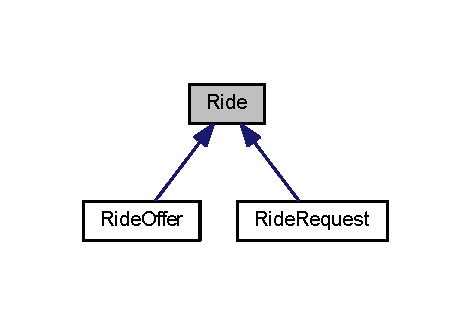
\includegraphics[width=226pt]{class_ride__inherit__graph}
\end{center}
\end{figure}


Collaboration diagram for Ride\+:
\nopagebreak
\begin{figure}[H]
\begin{center}
\leavevmode
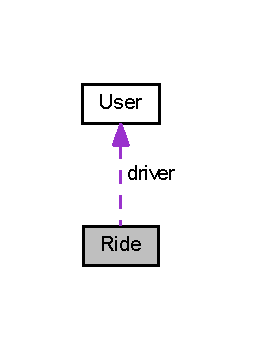
\includegraphics[width=124pt]{class_ride__coll__graph}
\end{center}
\end{figure}
\subsection*{Public Member Functions}
\begin{DoxyCompactItemize}
\item 
\hyperlink{class_ride_aef9cd8f2760f8e0b46eb268e69b007b9}{Ride} ()
\item 
\hyperlink{class_ride_a7642ec84a4f8522c58179962b142b276}{Ride} (uint departure\+Place, uint arrival\+Place, time\+\_\+t departure\+Time, time\+\_\+t departure\+Tolerance, time\+\_\+t arrival\+Tolerance, int no\+Seats)
\item 
virtual \hyperlink{class_ride_a51b5edd7f67bf27f5225d7e2c211c34d}{$\sim$\+Ride} ()
\item 
time\+\_\+t \hyperlink{class_ride_a7e031c140104824a87bc3664354a8d8b}{get\+Arrival\+Tolerance} () const 
\item 
time\+\_\+t \hyperlink{class_ride_a15b59e580fc86bba03302c1b14c0e733}{get\+Departure\+Time} () const 
\item 
time\+\_\+t \hyperlink{class_ride_a09d280e7b7be35d8c1957316b1fdfa53}{get\+Departure\+Tolerance} () const 
\item 
time\+\_\+t \hyperlink{class_ride_a498db4e46f6520b747a18156855ecd27}{get\+Estimated\+Arrival} () const 
\item 
int \hyperlink{class_ride_ac6ce2ae3098bf408b70ca71ecdfa1278}{get\+No\+Seats} () const 
\item 
uint \hyperlink{class_ride_a50e27ef44b2bb35fb5da873f89fc1990}{get\+Arrival\+Place} () const 
\item 
uint \hyperlink{class_ride_af49465a0f4c2f9eb896f8c102b1d5c1d}{get\+Departure\+Place} () const 
\end{DoxyCompactItemize}
\subsection*{Protected Attributes}
\begin{DoxyCompactItemize}
\item 
\hypertarget{class_ride_a176632238cfffb2d7fc889d233261fa0}{}uint {\bfseries departure\+Place}\label{class_ride_a176632238cfffb2d7fc889d233261fa0}

\item 
\hypertarget{class_ride_a9d3d96a9aeb76232bc07c52461cdc4ac}{}uint {\bfseries arrival\+Place}\label{class_ride_a9d3d96a9aeb76232bc07c52461cdc4ac}

\item 
\hypertarget{class_ride_ac3dd5b37d7ba828e6635a944425e6ace}{}time\+\_\+t {\bfseries departure\+Time}\label{class_ride_ac3dd5b37d7ba828e6635a944425e6ace}

\item 
\hypertarget{class_ride_ad4e0009e20129189e804b8cf7ad1766a}{}time\+\_\+t {\bfseries estimated\+Arrival}\label{class_ride_ad4e0009e20129189e804b8cf7ad1766a}

\item 
\hypertarget{class_ride_a668eeee90fb137d28ca2ce84345237bd}{}time\+\_\+t {\bfseries departure\+Tolerance}\label{class_ride_a668eeee90fb137d28ca2ce84345237bd}

\item 
\hypertarget{class_ride_ab6932b92492a60844ac831380ebf2e0d}{}time\+\_\+t {\bfseries arrival\+Tolerance}\label{class_ride_ab6932b92492a60844ac831380ebf2e0d}

\item 
\hypertarget{class_ride_a3e8ba79aefe64707fabfec0eed092784}{}int {\bfseries no\+Seats}\label{class_ride_a3e8ba79aefe64707fabfec0eed092784}

\item 
\hypertarget{class_ride_ad3855a5fce1f26c871ae3c70dfee6137}{}\hyperlink{class_user}{User} $\ast$ {\bfseries driver}\label{class_ride_ad3855a5fce1f26c871ae3c70dfee6137}

\item 
\hypertarget{class_ride_a0b0d7418f91b2991c199901b6cf48801}{}vector$<$ \hyperlink{class_user}{User} $\ast$ $>$ {\bfseries hitchhikers}\label{class_ride_a0b0d7418f91b2991c199901b6cf48801}

\end{DoxyCompactItemize}


\subsection{Detailed Description}
ride requests, offers and completed rides 

\subsection{Constructor \& Destructor Documentation}
\hypertarget{class_ride_aef9cd8f2760f8e0b46eb268e69b007b9}{}\index{Ride@{Ride}!Ride@{Ride}}
\index{Ride@{Ride}!Ride@{Ride}}
\subsubsection[{Ride()}]{\setlength{\rightskip}{0pt plus 5cm}Ride\+::\+Ride (
\begin{DoxyParamCaption}
{}
\end{DoxyParamCaption}
)\hspace{0.3cm}{\ttfamily [inline]}}\label{class_ride_aef9cd8f2760f8e0b46eb268e69b007b9}
Class default Constructor \hypertarget{class_ride_a7642ec84a4f8522c58179962b142b276}{}\index{Ride@{Ride}!Ride@{Ride}}
\index{Ride@{Ride}!Ride@{Ride}}
\subsubsection[{Ride(uint departure\+Place, uint arrival\+Place, time\+\_\+t departure\+Time, time\+\_\+t departure\+Tolerance, time\+\_\+t arrival\+Tolerance, int no\+Seats)}]{\setlength{\rightskip}{0pt plus 5cm}Ride\+::\+Ride (
\begin{DoxyParamCaption}
\item[{uint}]{departure\+Place, }
\item[{uint}]{arrival\+Place, }
\item[{time\+\_\+t}]{departure\+Time, }
\item[{time\+\_\+t}]{departure\+Tolerance, }
\item[{time\+\_\+t}]{arrival\+Tolerance, }
\item[{int}]{no\+Seats}
\end{DoxyParamCaption}
)}\label{class_ride_a7642ec84a4f8522c58179962b142b276}
Class base constructor \hypertarget{class_ride_a51b5edd7f67bf27f5225d7e2c211c34d}{}\index{Ride@{Ride}!````~Ride@{$\sim$\+Ride}}
\index{````~Ride@{$\sim$\+Ride}!Ride@{Ride}}
\subsubsection[{$\sim$\+Ride()}]{\setlength{\rightskip}{0pt plus 5cm}Ride\+::$\sim$\+Ride (
\begin{DoxyParamCaption}
{}
\end{DoxyParamCaption}
)\hspace{0.3cm}{\ttfamily [virtual]}}\label{class_ride_a51b5edd7f67bf27f5225d7e2c211c34d}
Class default destructor 

\subsection{Member Function Documentation}
\hypertarget{class_ride_a50e27ef44b2bb35fb5da873f89fc1990}{}\index{Ride@{Ride}!get\+Arrival\+Place@{get\+Arrival\+Place}}
\index{get\+Arrival\+Place@{get\+Arrival\+Place}!Ride@{Ride}}
\subsubsection[{get\+Arrival\+Place() const }]{\setlength{\rightskip}{0pt plus 5cm}uint Ride\+::get\+Arrival\+Place (
\begin{DoxyParamCaption}
{}
\end{DoxyParamCaption}
) const\hspace{0.3cm}{\ttfamily [inline]}}\label{class_ride_a50e27ef44b2bb35fb5da873f89fc1990}
\begin{DoxyReturn}{Returns}
place of arrival (inode) 
\end{DoxyReturn}
\hypertarget{class_ride_a7e031c140104824a87bc3664354a8d8b}{}\index{Ride@{Ride}!get\+Arrival\+Tolerance@{get\+Arrival\+Tolerance}}
\index{get\+Arrival\+Tolerance@{get\+Arrival\+Tolerance}!Ride@{Ride}}
\subsubsection[{get\+Arrival\+Tolerance() const }]{\setlength{\rightskip}{0pt plus 5cm}time\+\_\+t Ride\+::get\+Arrival\+Tolerance (
\begin{DoxyParamCaption}
{}
\end{DoxyParamCaption}
) const\hspace{0.3cm}{\ttfamily [inline]}}\label{class_ride_a7e031c140104824a87bc3664354a8d8b}
\begin{DoxyReturn}{Returns}
tolerance time for arrival 
\end{DoxyReturn}
\hypertarget{class_ride_af49465a0f4c2f9eb896f8c102b1d5c1d}{}\index{Ride@{Ride}!get\+Departure\+Place@{get\+Departure\+Place}}
\index{get\+Departure\+Place@{get\+Departure\+Place}!Ride@{Ride}}
\subsubsection[{get\+Departure\+Place() const }]{\setlength{\rightskip}{0pt plus 5cm}uint Ride\+::get\+Departure\+Place (
\begin{DoxyParamCaption}
{}
\end{DoxyParamCaption}
) const\hspace{0.3cm}{\ttfamily [inline]}}\label{class_ride_af49465a0f4c2f9eb896f8c102b1d5c1d}
\begin{DoxyReturn}{Returns}
place of departure (inode) 
\end{DoxyReturn}
\hypertarget{class_ride_a15b59e580fc86bba03302c1b14c0e733}{}\index{Ride@{Ride}!get\+Departure\+Time@{get\+Departure\+Time}}
\index{get\+Departure\+Time@{get\+Departure\+Time}!Ride@{Ride}}
\subsubsection[{get\+Departure\+Time() const }]{\setlength{\rightskip}{0pt plus 5cm}time\+\_\+t Ride\+::get\+Departure\+Time (
\begin{DoxyParamCaption}
{}
\end{DoxyParamCaption}
) const\hspace{0.3cm}{\ttfamily [inline]}}\label{class_ride_a15b59e580fc86bba03302c1b14c0e733}
\begin{DoxyReturn}{Returns}
departure date 
\end{DoxyReturn}
\hypertarget{class_ride_a09d280e7b7be35d8c1957316b1fdfa53}{}\index{Ride@{Ride}!get\+Departure\+Tolerance@{get\+Departure\+Tolerance}}
\index{get\+Departure\+Tolerance@{get\+Departure\+Tolerance}!Ride@{Ride}}
\subsubsection[{get\+Departure\+Tolerance() const }]{\setlength{\rightskip}{0pt plus 5cm}time\+\_\+t Ride\+::get\+Departure\+Tolerance (
\begin{DoxyParamCaption}
{}
\end{DoxyParamCaption}
) const\hspace{0.3cm}{\ttfamily [inline]}}\label{class_ride_a09d280e7b7be35d8c1957316b1fdfa53}
\begin{DoxyReturn}{Returns}
tolerance time for departure 
\end{DoxyReturn}
\hypertarget{class_ride_a498db4e46f6520b747a18156855ecd27}{}\index{Ride@{Ride}!get\+Estimated\+Arrival@{get\+Estimated\+Arrival}}
\index{get\+Estimated\+Arrival@{get\+Estimated\+Arrival}!Ride@{Ride}}
\subsubsection[{get\+Estimated\+Arrival() const }]{\setlength{\rightskip}{0pt plus 5cm}time\+\_\+t Ride\+::get\+Estimated\+Arrival (
\begin{DoxyParamCaption}
{}
\end{DoxyParamCaption}
) const\hspace{0.3cm}{\ttfamily [inline]}}\label{class_ride_a498db4e46f6520b747a18156855ecd27}
\begin{DoxyReturn}{Returns}
estimated time of arrival 
\end{DoxyReturn}
\hypertarget{class_ride_ac6ce2ae3098bf408b70ca71ecdfa1278}{}\index{Ride@{Ride}!get\+No\+Seats@{get\+No\+Seats}}
\index{get\+No\+Seats@{get\+No\+Seats}!Ride@{Ride}}
\subsubsection[{get\+No\+Seats() const }]{\setlength{\rightskip}{0pt plus 5cm}int Ride\+::get\+No\+Seats (
\begin{DoxyParamCaption}
{}
\end{DoxyParamCaption}
) const\hspace{0.3cm}{\ttfamily [inline]}}\label{class_ride_ac6ce2ae3098bf408b70ca71ecdfa1278}
\begin{DoxyReturn}{Returns}
number of seats 
\end{DoxyReturn}


The documentation for this class was generated from the following files\+:\begin{DoxyCompactItemize}
\item 
C\+:/\+Users/\+Inês/workspace/cal\+\_\+proj\+\_\+1/src/Ride.\+h\item 
C\+:/\+Users/\+Inês/workspace/cal\+\_\+proj\+\_\+1/src/Ride.\+cpp\end{DoxyCompactItemize}

\hypertarget{class_ride_completed}{}\section{Ride\+Completed Class Reference}
\label{class_ride_completed}\index{Ride\+Completed@{Ride\+Completed}}
\subsection*{Public Member Functions}
\begin{DoxyCompactItemize}
\item 
\hyperlink{class_ride_completed_a6cdeccf0aea565f56f77459cc75847c4}{Ride\+Completed} (\hyperlink{class_ride_offer}{Ride\+Offer} $\ast$ride\+Offer)
\item 
virtual \hyperlink{class_ride_completed_acee497903e9f19567cc931a0c57ec9c6}{$\sim$\+Ride\+Completed} ()
\end{DoxyCompactItemize}


\subsection{Detailed Description}
of rides that were matched 

\subsection{Constructor \& Destructor Documentation}
\index{Ride\+Completed@{Ride\+Completed}!Ride\+Completed@{Ride\+Completed}}
\index{Ride\+Completed@{Ride\+Completed}!Ride\+Completed@{Ride\+Completed}}
\subsubsection[{\texorpdfstring{Ride\+Completed(\+Ride\+Offer $\ast$ride\+Offer)}{RideCompleted(RideOffer *rideOffer)}}]{\setlength{\rightskip}{0pt plus 5cm}Ride\+Completed\+::\+Ride\+Completed (
\begin{DoxyParamCaption}
\item[{{\bf Ride\+Offer} $\ast$}]{ride\+Offer}
\end{DoxyParamCaption}
)}\hypertarget{class_ride_completed_a6cdeccf0aea565f56f77459cc75847c4}{}\label{class_ride_completed_a6cdeccf0aea565f56f77459cc75847c4}
Class base constructor \index{Ride\+Completed@{Ride\+Completed}!````~Ride\+Completed@{$\sim$\+Ride\+Completed}}
\index{````~Ride\+Completed@{$\sim$\+Ride\+Completed}!Ride\+Completed@{Ride\+Completed}}
\subsubsection[{\texorpdfstring{$\sim$\+Ride\+Completed()}{~RideCompleted()}}]{\setlength{\rightskip}{0pt plus 5cm}Ride\+Completed\+::$\sim$\+Ride\+Completed (
\begin{DoxyParamCaption}
{}
\end{DoxyParamCaption}
)\hspace{0.3cm}{\ttfamily [virtual]}}\hypertarget{class_ride_completed_acee497903e9f19567cc931a0c57ec9c6}{}\label{class_ride_completed_acee497903e9f19567cc931a0c57ec9c6}
Class default destructor 

The documentation for this class was generated from the following files\+:\begin{DoxyCompactItemize}
\item 
src/Ride\+Completed.\+h\item 
src/Ride\+Completed.\+cpp\end{DoxyCompactItemize}

\hypertarget{class_ride_offer}{}\section{Ride\+Offer Class Reference}
\label{class_ride_offer}\index{Ride\+Offer@{Ride\+Offer}}


Inheritance diagram for Ride\+Offer\+:
\nopagebreak
\begin{figure}[H]
\begin{center}
\leavevmode
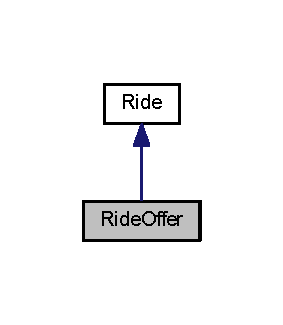
\includegraphics[width=136pt]{class_ride_offer__inherit__graph}
\end{center}
\end{figure}


Collaboration diagram for Ride\+Offer\+:
\nopagebreak
\begin{figure}[H]
\begin{center}
\leavevmode
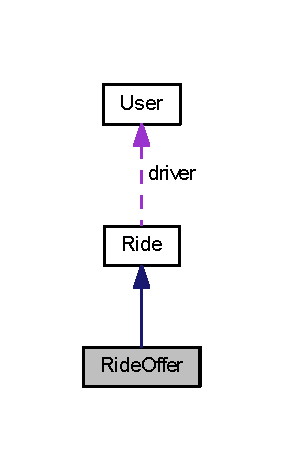
\includegraphics[width=136pt]{class_ride_offer__coll__graph}
\end{center}
\end{figure}
\subsection*{Public Member Functions}
\begin{DoxyCompactItemize}
\item 
\hypertarget{class_ride_offer_ade002d578a8ee317d34c88d5b4b5e2d7}{}{\bfseries Ride\+Offer} (uint departure\+Place, uint arrival\+Place, time\+\_\+t departure\+Time, time\+\_\+t departure\+Tolerance, time\+\_\+t arrival\+Tolerance, int no\+Seats, \hyperlink{class_user}{User} $\ast$driver)\label{class_ride_offer_ade002d578a8ee317d34c88d5b4b5e2d7}

\item 
\hypertarget{class_ride_offer_a145cf12bbda55809eb41740cbd45a6f5}{}void {\bfseries decrease\+No\+Seats} (uint no\+Seats)\label{class_ride_offer_a145cf12bbda55809eb41740cbd45a6f5}

\item 
\hypertarget{class_ride_offer_a62e995e6e3cc7aaa074d2a9f69329212}{}const vector$<$ \hyperlink{class_ride_request}{Ride\+Request} $>$ \& {\bfseries get\+Requests} () const \label{class_ride_offer_a62e995e6e3cc7aaa074d2a9f69329212}

\item 
\hypertarget{class_ride_offer_aa03bcf9a56b427b96ca09f55e26c5e9c}{}const std\+::list$<$ unsigned int $>$ \& {\bfseries get\+Route} () const \label{class_ride_offer_aa03bcf9a56b427b96ca09f55e26c5e9c}

\item 
\hypertarget{class_ride_offer_a173345d8bc9af6b0d951f8202aab0fef}{}void {\bfseries set\+Route} (const std\+::list$<$ unsigned int $>$ \&route)\label{class_ride_offer_a173345d8bc9af6b0d951f8202aab0fef}

\item 
\hypertarget{class_ride_offer_a0dc50af57fdea2e2869e4414e7bb124c}{}void {\bfseries add\+Request} (\hyperlink{class_ride_request}{Ride\+Request} request)\label{class_ride_offer_a0dc50af57fdea2e2869e4414e7bb124c}

\end{DoxyCompactItemize}
\subsection*{Additional Inherited Members}


The documentation for this class was generated from the following files\+:\begin{DoxyCompactItemize}
\item 
C\+:/\+Users/\+Inês/workspace/cal\+\_\+proj\+\_\+1/src/Ride\+Offer.\+h\item 
C\+:/\+Users/\+Inês/workspace/cal\+\_\+proj\+\_\+1/src/Ride\+Offer.\+cpp\end{DoxyCompactItemize}

\hypertarget{class_ride_request}{}\section{Ride\+Request Class Reference}
\label{class_ride_request}\index{Ride\+Request@{Ride\+Request}}


Inheritance diagram for Ride\+Request\+:\nopagebreak
\begin{figure}[H]
\begin{center}
\leavevmode
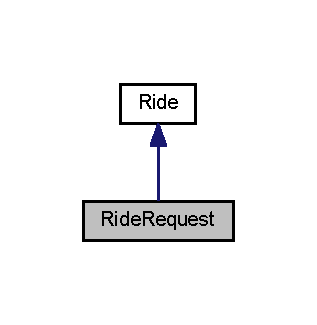
\includegraphics[width=152pt]{class_ride_request__inherit__graph}
\end{center}
\end{figure}


Collaboration diagram for Ride\+Request\+:\nopagebreak
\begin{figure}[H]
\begin{center}
\leavevmode
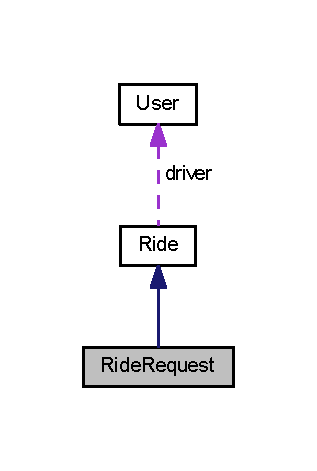
\includegraphics[width=152pt]{class_ride_request__coll__graph}
\end{center}
\end{figure}
\subsection*{Public Member Functions}
\begin{DoxyCompactItemize}
\item 
\hyperlink{class_ride_request_a58874aa113243ac8e5e6a2bf68a96037}{Ride\+Request} (uint departure\+Place, uint arrival\+Place, time\+\_\+t departure\+Time, time\+\_\+t departure\+Tolerance, time\+\_\+t arrival\+Tolerance, int no\+Seats, \hyperlink{class_user}{User} $\ast$hitchhiker)
\item 
virtual \hyperlink{class_ride_request_a0c37241ff14f6c423ca576159e3d8b19}{$\sim$\+Ride\+Request} ()
\end{DoxyCompactItemize}
\subsection*{Friends}
\begin{DoxyCompactItemize}
\item 
ostream \& {\bfseries operator$<$$<$} (ostream \&os, const \hyperlink{class_ride_request}{Ride\+Request} \&request)\hypertarget{class_ride_request_a8c8f6e260e585c5e323e35eefa59f779}{}\label{class_ride_request_a8c8f6e260e585c5e323e35eefa59f779}

\end{DoxyCompactItemize}
\subsection*{Additional Inherited Members}


\subsection{Detailed Description}
of ride offers

of ride requests 

\subsection{Constructor \& Destructor Documentation}
\index{Ride\+Request@{Ride\+Request}!Ride\+Request@{Ride\+Request}}
\index{Ride\+Request@{Ride\+Request}!Ride\+Request@{Ride\+Request}}
\subsubsection[{\texorpdfstring{Ride\+Request(uint departure\+Place, uint arrival\+Place, time\+\_\+t departure\+Time, time\+\_\+t departure\+Tolerance, time\+\_\+t arrival\+Tolerance, int no\+Seats, User $\ast$hitchhiker)}{RideRequest(uint departurePlace, uint arrivalPlace, time_t departureTime, time_t departureTolerance, time_t arrivalTolerance, int noSeats, User *hitchhiker)}}]{\setlength{\rightskip}{0pt plus 5cm}Ride\+Request\+::\+Ride\+Request (
\begin{DoxyParamCaption}
\item[{uint}]{departure\+Place, }
\item[{uint}]{arrival\+Place, }
\item[{time\+\_\+t}]{departure\+Time, }
\item[{time\+\_\+t}]{departure\+Tolerance, }
\item[{time\+\_\+t}]{arrival\+Tolerance, }
\item[{int}]{no\+Seats, }
\item[{{\bf User} $\ast$}]{hitchhiker}
\end{DoxyParamCaption}
)}\hypertarget{class_ride_request_a58874aa113243ac8e5e6a2bf68a96037}{}\label{class_ride_request_a58874aa113243ac8e5e6a2bf68a96037}
Class base constructor \index{Ride\+Request@{Ride\+Request}!````~Ride\+Request@{$\sim$\+Ride\+Request}}
\index{````~Ride\+Request@{$\sim$\+Ride\+Request}!Ride\+Request@{Ride\+Request}}
\subsubsection[{\texorpdfstring{$\sim$\+Ride\+Request()}{~RideRequest()}}]{\setlength{\rightskip}{0pt plus 5cm}Ride\+Request\+::$\sim$\+Ride\+Request (
\begin{DoxyParamCaption}
{}
\end{DoxyParamCaption}
)\hspace{0.3cm}{\ttfamily [virtual]}}\hypertarget{class_ride_request_a0c37241ff14f6c423ca576159e3d8b19}{}\label{class_ride_request_a0c37241ff14f6c423ca576159e3d8b19}
Class default destructor 

The documentation for this class was generated from the following files\+:\begin{DoxyCompactItemize}
\item 
src/Ride\+Request.\+h\item 
src/Ride\+Request.\+cpp\end{DoxyCompactItemize}

\hypertarget{class_road}{}\section{Road Class Reference}
\label{class_road}\index{Road@{Road}}
\subsection*{Public Member Functions}
\begin{DoxyCompactItemize}
\item 
\hyperlink{class_road_ab2d4cc8a9411ffb084af289e12d11c7b}{Road} (string name, bool two\+Way)
\item 
const string \& \hyperlink{class_road_a7420713cc7c3c5197a5e14b53f1fc5bc}{get\+Name} () const 
\item 
bool \hyperlink{class_road_a6a1b16571a08fc381d07ba4d996886d9}{is\+Two\+Way} () const 
\item 
void \hyperlink{class_road_add4001611c0f0c96823ca83682ec0999}{add\+Crossroad} (\hyperlink{class_crossroad}{Crossroad} $\ast$c)
\item 
vector$<$ \hyperlink{class_crossroad}{Crossroad} $\ast$ $>$ \hyperlink{class_road_af48bfda2527f0821540e5464c0d753fc}{get\+Crossroads} ()
\item 
unsigned int \hyperlink{class_road_afb61f123b83f3b5833112ce585dc66c6}{get\+Node\+Id} (string road\+Name, double door\+Number)
\end{DoxyCompactItemize}


\subsection{Detailed Description}
a given real world road 

\subsection{Constructor \& Destructor Documentation}
\index{Road@{Road}!Road@{Road}}
\index{Road@{Road}!Road@{Road}}
\subsubsection[{\texorpdfstring{Road(string name, bool two\+Way)}{Road(string name, bool twoWay)}}]{\setlength{\rightskip}{0pt plus 5cm}Road\+::\+Road (
\begin{DoxyParamCaption}
\item[{string}]{name, }
\item[{bool}]{two\+Way}
\end{DoxyParamCaption}
)\hspace{0.3cm}{\ttfamily [inline]}}\hypertarget{class_road_ab2d4cc8a9411ffb084af289e12d11c7b}{}\label{class_road_ab2d4cc8a9411ffb084af289e12d11c7b}
Class base constructor 

\subsection{Member Function Documentation}
\index{Road@{Road}!add\+Crossroad@{add\+Crossroad}}
\index{add\+Crossroad@{add\+Crossroad}!Road@{Road}}
\subsubsection[{\texorpdfstring{add\+Crossroad(\+Crossroad $\ast$c)}{addCrossroad(Crossroad *c)}}]{\setlength{\rightskip}{0pt plus 5cm}void Road\+::add\+Crossroad (
\begin{DoxyParamCaption}
\item[{{\bf Crossroad} $\ast$}]{c}
\end{DoxyParamCaption}
)\hspace{0.3cm}{\ttfamily [inline]}}\hypertarget{class_road_add4001611c0f0c96823ca83682ec0999}{}\label{class_road_add4001611c0f0c96823ca83682ec0999}
Adds a crossroad to the road 
\begin{DoxyParams}{Parameters}
{\em c} & given crossroad \\
\hline
\end{DoxyParams}
\index{Road@{Road}!get\+Crossroads@{get\+Crossroads}}
\index{get\+Crossroads@{get\+Crossroads}!Road@{Road}}
\subsubsection[{\texorpdfstring{get\+Crossroads()}{getCrossroads()}}]{\setlength{\rightskip}{0pt plus 5cm}vector$<${\bf Crossroad}$\ast$$>$ Road\+::get\+Crossroads (
\begin{DoxyParamCaption}
{}
\end{DoxyParamCaption}
)\hspace{0.3cm}{\ttfamily [inline]}}\hypertarget{class_road_af48bfda2527f0821540e5464c0d753fc}{}\label{class_road_af48bfda2527f0821540e5464c0d753fc}
\begin{DoxyReturn}{Returns}
the vector of crossroads 
\end{DoxyReturn}
\index{Road@{Road}!get\+Name@{get\+Name}}
\index{get\+Name@{get\+Name}!Road@{Road}}
\subsubsection[{\texorpdfstring{get\+Name() const }{getName() const }}]{\setlength{\rightskip}{0pt plus 5cm}const string\& Road\+::get\+Name (
\begin{DoxyParamCaption}
{}
\end{DoxyParamCaption}
) const\hspace{0.3cm}{\ttfamily [inline]}}\hypertarget{class_road_a7420713cc7c3c5197a5e14b53f1fc5bc}{}\label{class_road_a7420713cc7c3c5197a5e14b53f1fc5bc}
\begin{DoxyReturn}{Returns}
the road name 
\end{DoxyReturn}
\index{Road@{Road}!get\+Node\+Id@{get\+Node\+Id}}
\index{get\+Node\+Id@{get\+Node\+Id}!Road@{Road}}
\subsubsection[{\texorpdfstring{get\+Node\+Id(string road\+Name, double door\+Number)}{getNodeId(string roadName, double doorNumber)}}]{\setlength{\rightskip}{0pt plus 5cm}unsigned int Road\+::get\+Node\+Id (
\begin{DoxyParamCaption}
\item[{string}]{road\+Name, }
\item[{double}]{door\+Number}
\end{DoxyParamCaption}
)\hspace{0.3cm}{\ttfamily [inline]}}\hypertarget{class_road_afb61f123b83f3b5833112ce585dc66c6}{}\label{class_road_afb61f123b83f3b5833112ce585dc66c6}
Gets node id for a given road name and door number 
\begin{DoxyParams}{Parameters}
{\em road\+Name} & given road name \\
\hline
{\em door\+Number} & given door number \\
\hline
\end{DoxyParams}
\begin{DoxyReturn}{Returns}
node id 
\end{DoxyReturn}
\index{Road@{Road}!is\+Two\+Way@{is\+Two\+Way}}
\index{is\+Two\+Way@{is\+Two\+Way}!Road@{Road}}
\subsubsection[{\texorpdfstring{is\+Two\+Way() const }{isTwoWay() const }}]{\setlength{\rightskip}{0pt plus 5cm}bool Road\+::is\+Two\+Way (
\begin{DoxyParamCaption}
{}
\end{DoxyParamCaption}
) const\hspace{0.3cm}{\ttfamily [inline]}}\hypertarget{class_road_a6a1b16571a08fc381d07ba4d996886d9}{}\label{class_road_a6a1b16571a08fc381d07ba4d996886d9}
\begin{DoxyReturn}{Returns}
true if the road can be travelled in both directions, false if it can\textquotesingle{}t 
\end{DoxyReturn}


The documentation for this class was generated from the following file\+:\begin{DoxyCompactItemize}
\item 
src/Road.\+h\end{DoxyCompactItemize}

\hypertarget{class_road_map}{}\section{Road\+Map Class Reference}
\label{class_road_map}\index{Road\+Map@{Road\+Map}}


Inheritance diagram for Road\+Map\+:
\nopagebreak
\begin{figure}[H]
\begin{center}
\leavevmode
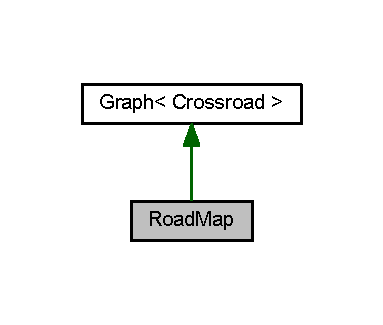
\includegraphics[width=184pt]{class_road_map__inherit__graph}
\end{center}
\end{figure}


Collaboration diagram for Road\+Map\+:
\nopagebreak
\begin{figure}[H]
\begin{center}
\leavevmode
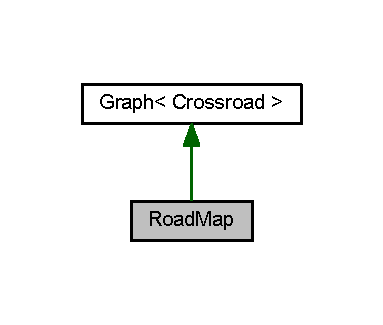
\includegraphics[width=184pt]{class_road_map__coll__graph}
\end{center}
\end{figure}
\subsection*{Public Member Functions}
\begin{DoxyCompactItemize}
\item 
void \hyperlink{class_road_map_a3a2719b8e8cbbd197b94092a33376666}{reset\+Map} ()
\item 
void \hyperlink{class_road_map_a8783164e6e3f029e2ca1bac4ee620db5}{view\+Map} ()
\item 
void \hyperlink{class_road_map_a51dda1085cb948aef5593530223aa202}{best\+Path} (uint new\+Src, uint new\+Dest, list$<$ uint $>$ \&old\+Path, list$<$ double $>$ \&dist)
\item 
bool \hyperlink{class_road_map_a6e25c8aefc49316e95c3eb3111d06151}{insert\+New\+Dest} (uint id\+\_\+src, uint id\+\_\+dest, list$<$ uint $>$ must\+Pass, list$<$ uint $>$ \&path, list$<$ double $>$ \&dist)
\item 
void \hyperlink{class_road_map_a00a0a45209179dae49cebd1c50908dd6}{insert\+New\+Src} (uint src\+Id, uint dest\+Id, uint new\+Src, list$<$ uint $>$ \&must\+Pass, list$<$ uint $>$ \&path, list$<$ double $>$ \&dist)
\item 
uint \hyperlink{class_road_map_aca51fa3ea3ae51d9790f186092fe9a29}{get\+Crossroad\+Id\+From\+Address} (string road\+Name, double door\+Number)
\item 
bool \hyperlink{class_road_map_aa1e10da727052cf0ca8c4a050e1c684b}{valid\+Crossroad\+Id} (uint id)
\item 
double \hyperlink{class_road_map_a9970c4e809908d7a3784b23666ec5d10}{get\+Dist} (uint src\+Id, uint dest\+Id)
\item 
vector$<$ string $>$ \hyperlink{class_road_map_acecd13293d634caa11afba05ec496233}{get\+Roads\+Passed} (list$<$ uint $>$ path)
\item 
void \hyperlink{class_road_map_a700ada8d9925f1322804e0d08a007ff1}{visualize\+Path} (list$<$ uint $>$ path)
\item 
\hyperlink{class_road_map_a4945159808914eb623e1abb3b9b63306}{$\sim$\+Road\+Map} ()
\end{DoxyCompactItemize}
\subsection*{Static Public Member Functions}
\begin{DoxyCompactItemize}
\item 
static \hyperlink{class_road_map}{Road\+Map} $\ast$ {\bfseries get\+Instance} ()\hypertarget{class_road_map_ad106d7b921a092b9375682a5ec475fae}{}\label{class_road_map_ad106d7b921a092b9375682a5ec475fae}

\end{DoxyCompactItemize}
\subsection*{Additional Inherited Members}


\subsection{Detailed Description}
\hyperlink{class_road}{Road} Map 

\subsection{Constructor \& Destructor Documentation}
\index{Road\+Map@{Road\+Map}!````~Road\+Map@{$\sim$\+Road\+Map}}
\index{````~Road\+Map@{$\sim$\+Road\+Map}!Road\+Map@{Road\+Map}}
\subsubsection[{\texorpdfstring{$\sim$\+Road\+Map()}{~RoadMap()}}]{\setlength{\rightskip}{0pt plus 5cm}Road\+Map\+::$\sim$\+Road\+Map (
\begin{DoxyParamCaption}
{}
\end{DoxyParamCaption}
)}\hypertarget{class_road_map_a4945159808914eb623e1abb3b9b63306}{}\label{class_road_map_a4945159808914eb623e1abb3b9b63306}
Default class destructor 

\subsection{Member Function Documentation}
\index{Road\+Map@{Road\+Map}!best\+Path@{best\+Path}}
\index{best\+Path@{best\+Path}!Road\+Map@{Road\+Map}}
\subsubsection[{\texorpdfstring{best\+Path(uint new\+Src, uint new\+Dest, list$<$ uint $>$ \&old\+Path, list$<$ double $>$ \&dist)}{bestPath(uint newSrc, uint newDest, list< uint > &oldPath, list< double > &dist)}}]{\setlength{\rightskip}{0pt plus 5cm}void Road\+Map\+::best\+Path (
\begin{DoxyParamCaption}
\item[{uint}]{new\+Src, }
\item[{uint}]{new\+Dest, }
\item[{list$<$ uint $>$ \&}]{old\+Path, }
\item[{list$<$ double $>$ \&}]{dist}
\end{DoxyParamCaption}
)}\hypertarget{class_road_map_a51dda1085cb948aef5593530223aa202}{}\label{class_road_map_a51dda1085cb948aef5593530223aa202}
Finds the best path given the current path and new 2 points \index{Road\+Map@{Road\+Map}!get\+Crossroad\+Id\+From\+Address@{get\+Crossroad\+Id\+From\+Address}}
\index{get\+Crossroad\+Id\+From\+Address@{get\+Crossroad\+Id\+From\+Address}!Road\+Map@{Road\+Map}}
\subsubsection[{\texorpdfstring{get\+Crossroad\+Id\+From\+Address(string road\+Name, double door\+Number)}{getCrossroadIdFromAddress(string roadName, double doorNumber)}}]{\setlength{\rightskip}{0pt plus 5cm}uint Road\+Map\+::get\+Crossroad\+Id\+From\+Address (
\begin{DoxyParamCaption}
\item[{string}]{road\+Name, }
\item[{double}]{door\+Number}
\end{DoxyParamCaption}
)}\hypertarget{class_road_map_aca51fa3ea3ae51d9790f186092fe9a29}{}\label{class_road_map_aca51fa3ea3ae51d9790f186092fe9a29}
Given an address and door number, returns the crossroad id \index{Road\+Map@{Road\+Map}!get\+Dist@{get\+Dist}}
\index{get\+Dist@{get\+Dist}!Road\+Map@{Road\+Map}}
\subsubsection[{\texorpdfstring{get\+Dist(uint src\+Id, uint dest\+Id)}{getDist(uint srcId, uint destId)}}]{\setlength{\rightskip}{0pt plus 5cm}double Road\+Map\+::get\+Dist (
\begin{DoxyParamCaption}
\item[{uint}]{src\+Id, }
\item[{uint}]{dest\+Id}
\end{DoxyParamCaption}
)}\hypertarget{class_road_map_a9970c4e809908d7a3784b23666ec5d10}{}\label{class_road_map_a9970c4e809908d7a3784b23666ec5d10}
\begin{DoxyReturn}{Returns}
the distance between two inodes 
\end{DoxyReturn}
\index{Road\+Map@{Road\+Map}!get\+Roads\+Passed@{get\+Roads\+Passed}}
\index{get\+Roads\+Passed@{get\+Roads\+Passed}!Road\+Map@{Road\+Map}}
\subsubsection[{\texorpdfstring{get\+Roads\+Passed(list$<$ uint $>$ path)}{getRoadsPassed(list< uint > path)}}]{\setlength{\rightskip}{0pt plus 5cm}vector$<$ string $>$ Road\+Map\+::get\+Roads\+Passed (
\begin{DoxyParamCaption}
\item[{list$<$ uint $>$}]{path}
\end{DoxyParamCaption}
)}\hypertarget{class_road_map_acecd13293d634caa11afba05ec496233}{}\label{class_road_map_acecd13293d634caa11afba05ec496233}

\begin{DoxyParams}{Parameters}
{\em path} & list of crossroad ids of given path \\
\hline
\end{DoxyParams}
\begin{DoxyReturn}{Returns}
the name of the roads passed in certain path 
\end{DoxyReturn}
\index{Road\+Map@{Road\+Map}!insert\+New\+Dest@{insert\+New\+Dest}}
\index{insert\+New\+Dest@{insert\+New\+Dest}!Road\+Map@{Road\+Map}}
\subsubsection[{\texorpdfstring{insert\+New\+Dest(uint id\+\_\+src, uint id\+\_\+dest, list$<$ uint $>$ must\+Pass, list$<$ uint $>$ \&path, list$<$ double $>$ \&dist)}{insertNewDest(uint id_src, uint id_dest, list< uint > mustPass, list< uint > &path, list< double > &dist)}}]{\setlength{\rightskip}{0pt plus 5cm}bool Road\+Map\+::insert\+New\+Dest (
\begin{DoxyParamCaption}
\item[{uint}]{id\+\_\+src, }
\item[{uint}]{id\+\_\+dest, }
\item[{list$<$ uint $>$}]{must\+Pass, }
\item[{list$<$ uint $>$ \&}]{path, }
\item[{list$<$ double $>$ \&}]{dist}
\end{DoxyParamCaption}
)}\hypertarget{class_road_map_a6e25c8aefc49316e95c3eb3111d06151}{}\label{class_road_map_a6e25c8aefc49316e95c3eb3111d06151}
Inserts the new destination to pass by on the existing path \index{Road\+Map@{Road\+Map}!insert\+New\+Src@{insert\+New\+Src}}
\index{insert\+New\+Src@{insert\+New\+Src}!Road\+Map@{Road\+Map}}
\subsubsection[{\texorpdfstring{insert\+New\+Src(uint src\+Id, uint dest\+Id, uint new\+Src, list$<$ uint $>$ \&must\+Pass, list$<$ uint $>$ \&path, list$<$ double $>$ \&dist)}{insertNewSrc(uint srcId, uint destId, uint newSrc, list< uint > &mustPass, list< uint > &path, list< double > &dist)}}]{\setlength{\rightskip}{0pt plus 5cm}void Road\+Map\+::insert\+New\+Src (
\begin{DoxyParamCaption}
\item[{uint}]{src\+Id, }
\item[{uint}]{dest\+Id, }
\item[{uint}]{new\+Src, }
\item[{list$<$ uint $>$ \&}]{must\+Pass, }
\item[{list$<$ uint $>$ \&}]{path, }
\item[{list$<$ double $>$ \&}]{dist}
\end{DoxyParamCaption}
)}\hypertarget{class_road_map_a00a0a45209179dae49cebd1c50908dd6}{}\label{class_road_map_a00a0a45209179dae49cebd1c50908dd6}
Inserts the new point to pick-\/up a user to pass by on the existing path \index{Road\+Map@{Road\+Map}!reset\+Map@{reset\+Map}}
\index{reset\+Map@{reset\+Map}!Road\+Map@{Road\+Map}}
\subsubsection[{\texorpdfstring{reset\+Map()}{resetMap()}}]{\setlength{\rightskip}{0pt plus 5cm}void Road\+Map\+::reset\+Map (
\begin{DoxyParamCaption}
{}
\end{DoxyParamCaption}
)}\hypertarget{class_road_map_a3a2719b8e8cbbd197b94092a33376666}{}\label{class_road_map_a3a2719b8e8cbbd197b94092a33376666}
Resets map to its inicial condition \index{Road\+Map@{Road\+Map}!valid\+Crossroad\+Id@{valid\+Crossroad\+Id}}
\index{valid\+Crossroad\+Id@{valid\+Crossroad\+Id}!Road\+Map@{Road\+Map}}
\subsubsection[{\texorpdfstring{valid\+Crossroad\+Id(uint id)}{validCrossroadId(uint id)}}]{\setlength{\rightskip}{0pt plus 5cm}bool Road\+Map\+::valid\+Crossroad\+Id (
\begin{DoxyParamCaption}
\item[{uint}]{id}
\end{DoxyParamCaption}
)}\hypertarget{class_road_map_aa1e10da727052cf0ca8c4a050e1c684b}{}\label{class_road_map_aa1e10da727052cf0ca8c4a050e1c684b}
Given an id, checks if there is a crossroad with that id \index{Road\+Map@{Road\+Map}!view\+Map@{view\+Map}}
\index{view\+Map@{view\+Map}!Road\+Map@{Road\+Map}}
\subsubsection[{\texorpdfstring{view\+Map()}{viewMap()}}]{\setlength{\rightskip}{0pt plus 5cm}void Road\+Map\+::view\+Map (
\begin{DoxyParamCaption}
{}
\end{DoxyParamCaption}
)}\hypertarget{class_road_map_a8783164e6e3f029e2ca1bac4ee620db5}{}\label{class_road_map_a8783164e6e3f029e2ca1bac4ee620db5}
Shows the map on the screen \index{Road\+Map@{Road\+Map}!visualize\+Path@{visualize\+Path}}
\index{visualize\+Path@{visualize\+Path}!Road\+Map@{Road\+Map}}
\subsubsection[{\texorpdfstring{visualize\+Path(list$<$ uint $>$ path)}{visualizePath(list< uint > path)}}]{\setlength{\rightskip}{0pt plus 5cm}void Road\+Map\+::visualize\+Path (
\begin{DoxyParamCaption}
\item[{list$<$ uint $>$}]{path}
\end{DoxyParamCaption}
)}\hypertarget{class_road_map_a700ada8d9925f1322804e0d08a007ff1}{}\label{class_road_map_a700ada8d9925f1322804e0d08a007ff1}
Shows the given path on the graphviewer 

The documentation for this class was generated from the following files\+:\begin{DoxyCompactItemize}
\item 
src/Road\+Map.\+h\item 
src/Road\+Map.\+cpp\end{DoxyCompactItemize}

\hypertarget{class_user}{}\section{User Class Reference}
\label{class_user}\index{User@{User}}
\subsection*{Public Member Functions}
\begin{DoxyCompactItemize}
\item 
\hyperlink{class_user_a7d8f1de813351d98afcfe7f2daf41507}{User} (string name, string address)
\item 
int \hyperlink{class_user_ada4589ad6179f55dcb35ab5afdab78f5}{get\+User\+ID} () const 
\item 
const string \& \hyperlink{class_user_ad253dd3bf9b1effaab72e36e13e1d152}{get\+Name} () const 
\item 
const string \& \hyperlink{class_user_aa575209c344804d21452e6de006ef467}{get\+Address} () const 
\end{DoxyCompactItemize}
\subsection*{Friends}
\begin{DoxyCompactItemize}
\item 
bool {\bfseries operator==} (const \hyperlink{class_user}{User} \&u1, const \hyperlink{class_user}{User} \&u2)\hypertarget{class_user_af6f50d4046256c15aa6b2a061543bfbe}{}\label{class_user_af6f50d4046256c15aa6b2a061543bfbe}

\item 
ostream \& {\bfseries operator$<$$<$} (ostream \&os, const \hyperlink{class_user}{User} \&u)\hypertarget{class_user_a033c555cac168a4b631ea88982e171a8}{}\label{class_user_a033c555cac168a4b631ea88982e171a8}

\end{DoxyCompactItemize}


\subsection{Detailed Description}
user data and functionalities 

\subsection{Constructor \& Destructor Documentation}
\index{User@{User}!User@{User}}
\index{User@{User}!User@{User}}
\subsubsection[{\texorpdfstring{User(string name, string address)}{User(string name, string address)}}]{\setlength{\rightskip}{0pt plus 5cm}User\+::\+User (
\begin{DoxyParamCaption}
\item[{string}]{name, }
\item[{string}]{address}
\end{DoxyParamCaption}
)}\hypertarget{class_user_a7d8f1de813351d98afcfe7f2daf41507}{}\label{class_user_a7d8f1de813351d98afcfe7f2daf41507}
Class base constructor 

\subsection{Member Function Documentation}
\index{User@{User}!get\+Address@{get\+Address}}
\index{get\+Address@{get\+Address}!User@{User}}
\subsubsection[{\texorpdfstring{get\+Address() const }{getAddress() const }}]{\setlength{\rightskip}{0pt plus 5cm}const string\& User\+::get\+Address (
\begin{DoxyParamCaption}
{}
\end{DoxyParamCaption}
) const\hspace{0.3cm}{\ttfamily [inline]}}\hypertarget{class_user_aa575209c344804d21452e6de006ef467}{}\label{class_user_aa575209c344804d21452e6de006ef467}
\begin{DoxyReturn}{Returns}
user address 
\end{DoxyReturn}
\index{User@{User}!get\+Name@{get\+Name}}
\index{get\+Name@{get\+Name}!User@{User}}
\subsubsection[{\texorpdfstring{get\+Name() const }{getName() const }}]{\setlength{\rightskip}{0pt plus 5cm}const string\& User\+::get\+Name (
\begin{DoxyParamCaption}
{}
\end{DoxyParamCaption}
) const\hspace{0.3cm}{\ttfamily [inline]}}\hypertarget{class_user_ad253dd3bf9b1effaab72e36e13e1d152}{}\label{class_user_ad253dd3bf9b1effaab72e36e13e1d152}
\begin{DoxyReturn}{Returns}
user name 
\end{DoxyReturn}
\index{User@{User}!get\+User\+ID@{get\+User\+ID}}
\index{get\+User\+ID@{get\+User\+ID}!User@{User}}
\subsubsection[{\texorpdfstring{get\+User\+I\+D() const }{getUserID() const }}]{\setlength{\rightskip}{0pt plus 5cm}int User\+::get\+User\+ID (
\begin{DoxyParamCaption}
{}
\end{DoxyParamCaption}
) const\hspace{0.3cm}{\ttfamily [inline]}}\hypertarget{class_user_ada4589ad6179f55dcb35ab5afdab78f5}{}\label{class_user_ada4589ad6179f55dcb35ab5afdab78f5}
\begin{DoxyReturn}{Returns}
user ID 
\end{DoxyReturn}


The documentation for this class was generated from the following files\+:\begin{DoxyCompactItemize}
\item 
src/User.\+h\item 
src/User.\+cpp\end{DoxyCompactItemize}

\hypertarget{class_vertex}{}\section{Vertex$<$ T, U $>$ Class Template Reference}
\label{class_vertex}\index{Vertex$<$ T, U $>$@{Vertex$<$ T, U $>$}}


Collaboration diagram for Vertex$<$ T, U $>$\+:
\nopagebreak
\begin{figure}[H]
\begin{center}
\leavevmode
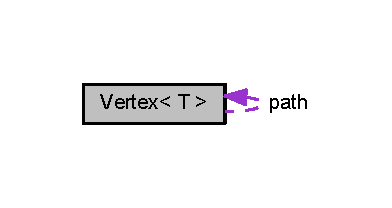
\includegraphics[width=188pt]{class_vertex__coll__graph}
\end{center}
\end{figure}
\subsection*{Public Member Functions}
\begin{DoxyCompactItemize}
\item 
{\bfseries Vertex} (T in)\hypertarget{class_vertex_a7376d289d627ca743c31ff81b8e6e2cc}{}\label{class_vertex_a7376d289d627ca743c31ff81b8e6e2cc}

\item 
void {\bfseries add\+Edge} (\hyperlink{class_vertex}{Vertex}$<$ T, U $>$ $\ast$dest, double w, U $\ast$info)\hypertarget{class_vertex_a1671c74e85d9f4fce8a51aafb8094656}{}\label{class_vertex_a1671c74e85d9f4fce8a51aafb8094656}

\item 
bool {\bfseries remove\+Edge\+To} (\hyperlink{class_vertex}{Vertex}$<$ T, U $>$ $\ast$d)\hypertarget{class_vertex_ad785fe108a5867370baf09ce04f15de7}{}\label{class_vertex_ad785fe108a5867370baf09ce04f15de7}

\item 
T {\bfseries get\+Info} () const \hypertarget{class_vertex_a94729f236fbeebf0febfc2b08a3806fa}{}\label{class_vertex_a94729f236fbeebf0febfc2b08a3806fa}

\item 
void {\bfseries set\+Info} (T info)\hypertarget{class_vertex_a63939669caca4a3990c1cda699c361d5}{}\label{class_vertex_a63939669caca4a3990c1cda699c361d5}

\item 
double {\bfseries get\+Dist} () const \hypertarget{class_vertex_a8a305cc552459bbfb4d2b394081a83a9}{}\label{class_vertex_a8a305cc552459bbfb4d2b394081a83a9}

\item 
int {\bfseries get\+Indegree} () const \hypertarget{class_vertex_a4665dac0df974a3eded2d7573e2ce042}{}\label{class_vertex_a4665dac0df974a3eded2d7573e2ce042}

\item 
vector$<$ \hyperlink{class_edge}{Edge}$<$ T, U $>$ $>$ {\bfseries get\+Adj} ()\hypertarget{class_vertex_a028d730c627918d3d452e5dc9b40b2fc}{}\label{class_vertex_a028d730c627918d3d452e5dc9b40b2fc}

\item 
bool {\bfseries operator$<$} (const \hyperlink{class_vertex}{Vertex}$<$ T, U $>$ vertex)\hypertarget{class_vertex_a46be891a4fe4a2c748211da700664dba}{}\label{class_vertex_a46be891a4fe4a2c748211da700664dba}

\end{DoxyCompactItemize}
\subsection*{Public Attributes}
\begin{DoxyCompactItemize}
\item 
\hyperlink{class_vertex}{Vertex} $\ast$ {\bfseries path}\hypertarget{class_vertex_a6166fbda36ae6a8e1d4fe69423c00e9d}{}\label{class_vertex_a6166fbda36ae6a8e1d4fe69423c00e9d}

\end{DoxyCompactItemize}
\subsection*{Friends}
\begin{DoxyCompactItemize}
\item 
class {\bfseries Graph$<$ T, U $>$}\hypertarget{class_vertex_a3a700cfc5d314381d768caf37b1108b9}{}\label{class_vertex_a3a700cfc5d314381d768caf37b1108b9}

\end{DoxyCompactItemize}


The documentation for this class was generated from the following file\+:\begin{DoxyCompactItemize}
\item 
src/Graph.\+h\end{DoxyCompactItemize}

\hypertarget{structvertex__greater__than}{}\section{vertex\+\_\+greater\+\_\+than$<$ T $>$ Struct Template Reference}
\label{structvertex__greater__than}\index{vertex\+\_\+greater\+\_\+than$<$ T $>$@{vertex\+\_\+greater\+\_\+than$<$ T $>$}}
\subsection*{Public Member Functions}
\begin{DoxyCompactItemize}
\item 
\hypertarget{structvertex__greater__than_af58940d572829488c2915ca53663631e}{}bool {\bfseries operator()} (\hyperlink{class_vertex}{Vertex}$<$ T $>$ $\ast$a, \hyperlink{class_vertex}{Vertex}$<$ T $>$ $\ast$b) const \label{structvertex__greater__than_af58940d572829488c2915ca53663631e}

\end{DoxyCompactItemize}


The documentation for this struct was generated from the following file\+:\begin{DoxyCompactItemize}
\item 
C\+:/\+Users/\+Inês/workspace/cal\+\_\+proj\+\_\+1/src/Graph.\+h\end{DoxyCompactItemize}

\hypertarget{class_wrong_file_parameters}{}\section{Wrong\+File\+Parameters Class Reference}
\label{class_wrong_file_parameters}\index{Wrong\+File\+Parameters@{Wrong\+File\+Parameters}}


The documentation for this class was generated from the following file\+:\begin{DoxyCompactItemize}
\item 
src/Exceptions.\+h\end{DoxyCompactItemize}

%--- End generated contents ---

% Index
\backmatter
\newpage
\phantomsection
\clearemptydoublepage
\addcontentsline{toc}{chapter}{Index}
\printindex

\end{document}
